\documentclass{article}
\usepackage{graphicx} % Required for inserting images
\usepackage[left=3cm, right=3cm, top=3cm, bottom=3cm]{geometry}
\usepackage{hyperref}
\usepackage{url}
\usepackage[titles]{tocloft}
\usepackage{amsmath}
\usepackage[czech]{babel}
\usepackage[utf8]{inputenc}

\usepackage{listings}
\usepackage[dvipsnames]{xcolor}
%\usepackage{amsmath}
\usepackage{mdframed}

\graphicspath{{figures/}}

\renewcommand{\lstlistlistingname}{Code Snippets}

\newcommand{\dd}{\ensuremath{\mathrm{d}}}
\newcommand{\diff}[2]{\ensuremath{\frac{\dd {#1}}{\dd {#2}}}}
\newcommand{\bv}[1]{\ensuremath{\mathbf{#1}}}
\newcommand{\ls}[1]{\lstinline{#1}}

\definecolor{codegreen}{rgb}{0,0.6,0}
\definecolor{codegray}{rgb}{0.5,0.5,0.5}
\definecolor{codepurple}{rgb}{0.58,0,0.82}
\definecolor{backcolour}{rgb}{0.95,0.95,0.92}
\definecolor{exercise}{gray}{0.9}
\definecolor{SIM}{cmyk}{0.1, 0, 0, 0}

\newcounter{exercise}
\newenvironment{exercise}[1][]%
    {\refstepcounter{exercise}%
    \begin{mdframed}[backgroundcolor=exercise,linecolor=white]%
    \textbf{Cvičení~\theexercise.} #1 \rmfamily}%
    {\medskip\end{mdframed}}

\newcommand{\listsyntax}{Python Jazykové Intermezza}
\newlistof{intermezzos}{synt}{\listsyntax}
\newcounter{syntax}
\newenvironment{syntax}[1][Syntax]%
    {\refstepcounter{syntax}%
    \addcontentsline{synt}{intermezzos}{#1}
    \begin{mdframed}[backgroundcolor=SIM,linecolor=white]%
    \textbf{Intermezzo~\thesyntax:} \textit{#1}}%
    {\medskip\end{mdframed}}

\lstdefinestyle{py}{
    backgroundcolor=\color{backcolour},
    commentstyle=\color{codegreen},
    keywordstyle=\color{magenta},
    numberstyle=\tiny\color{codegray},
    stringstyle=\color{codepurple},
    basicstyle=\ttfamily\footnotesize,
    breakatwhitespace=false,
    breaklines=true,
    captionpos=b,
    keepspaces=true,
    numbers=left,
    numbersep=5pt,
    showspaces=false,
    showstringspaces=false,
    showtabs=false,
    tabsize=2,
    language=Python
}
\lstset{style=py}

\title{NOFY080 poznámky k přednášce}
\author{Emil Varga}
\date{\today}

\begin{document}

\maketitle

\tableofcontents
\listofintermezzos
\lstlistoflistings

% Section 1: Setting up the environment
\newpage
\section{Setting up the environment}
Typical programming in python heavily relies on external packages, which can have different versions and dependencies. To avoid conflicts between different projects, it is recommended to use a virtual environment for each project. We will be using such virtual environment in this course to ensure a consistent development environment for everyone. Virtual environments are the recommended way to manage dependencies in Python projects.

To manage these virtual environments we will be using the open-source tool \verb|uv|, available from \url{https://github.com/astral-sh/uv}. If you have any version of Python already installed, you can install uv by simply running
\begin{lstlisting}
pip install uv
\end{lstlisting}
If you don't have Python installed, you can download it from \url{https://www.python.org/downloads/} and then use the above command or use the stand-alone installers on \url{https://github.com/astral-sh/uv}.

To test the installation, run in your command line
\begin{lstlisting}
uv --version
\end{lstlisting}
and something similar to \verb|uv 0.5.30| should appear.

Now we will create a project called \verb|NOFY080_2025| that will hold all the files related to this course, run
\begin{lstlisting}
uv init NOFY080_2025
\end{lstlisting}
which will create a new directory with the same name, with a simple "Hello World" python file, some additional files that \verb|uv| uses to track dependencies of your project and set up a git repository in it (you don't have to use git in this course, but those interested can learn some basics in Appendix~\ref{sec:git}).

Now change into the project directory
\begin{lstlisting}
cd NOFY080_2025
\end{lstlisting}
and add packages that we will need throughout this course
\begin{lstlisting}
uv add numpy scipy matplotlib
\end{lstlisting}
which will create the virtual environment and install the specified packages (a directory \verb|.venv| should appear in the project directory).

If you wanted to create a virtual environment without installing any packages, you could use the command
\begin{lstlisting}
uv venv <name of the virtual environment>
\end{lstlisting}

To activate the virtual environment, run the following command on Linux or Mac OS
\begin{lstlisting}
source .venv/bin/activate
\end{lstlisting}
and on Windows
\begin{lstlisting}
.venv\Scripts\activate
\end{lstlisting}

Now, when you run \verb|python|, the virtual environment version will be run, rather than your system version. To deactivate the virtual environment simply run \verb|deactivate|.

\subsection{Running Python code}
Python is an interpreted language that does not need to be compiled before it is run. We save Python code in text files with \verb|.py| file extension or in so-called Jupyter notebooks (file extension \verb|.ipynb|).

To test our installation, create a new Python file (a text file with suffix \verb|.py|) \verb|test.py| in our project directory with the following content
\begin{lstlisting}
import matplotlib.pyplot as plt

plt.plot([1, 2, 3], [4, 5, 6], '-o')
plt.show()
\end{lstlisting}
To run it, you can either manually activate the virtual environment and run it using
\verb|python test.py| or use \verb|uv run test.py|. A simple graph should appear. In the rest of these lecture notes, whenever we invoke \verb|python| command from the command line, we mean the one in the virtual environment.

To run Python code directly without saving it to a file, open a suitable terminal and type in \verb|python| and a prompt like
\begin{lstlisting}
    >>>
\end{lstlisting}
will appear. This is the Read-Evaluate-Print-Loop (REPL), any code entered will be run and the result printed on the screen. To exit enter \verb|quit()|. To execute a file \verb|myfile.py|, first navigate to its directory and then run it simply with \verb|python myfile.py| (note that if you have your virtual environment activated, the actual python script does not have to be located in your project directory).

\begin{exercise}
    Create a textfile \verb|hello.py| which contains a single line
    \begin{lstlisting}
        print("Hello world!")
    \end{lstlisting}
    and then run this file.
\end{exercise}

Sometimes we do not want the Python interpreter to quit immediately after finishing running our program (e.g., we want to inspect variables created during the program run), this can be done using \verb|python -i file.py|, \verb|-i| stands for \emph{interactive}. Alternatively, a more user-friendly (color-coded syntax, auto-completion, etc.) version of the interactive python REPL can be invoked using \verb|ipython| (or \verb|ipython3|, depending on your installation), which can also be used to interactively run files using \verb|ipython3 -i myfile.py|

\subsection{A quick note on text editors}
Any text editor can be used to write Python code, including the default Windows Notepad. However, it is beneficial to your mental health to use at least something with syntax highlighting, such as Notepad++, or a more feature-rich editor such as VS Code or Spyder where you can run your file without switching to a terminal. In this course, I recommend using VS Code with Python extension installed, because it makes working with virtual environments easier. Opening a directory in VS Code will automatically detect the virtual environment and use it when the file is run, the name of the virtual environment currently used is indicated in the bottom right corner (highligted in red)
\begin{center}
    \includegraphics[width=0.9\linewidth]{vscode.png}
\end{center}

Working with environments in Spyder is somewhat more involved, see the guide \href{https://github.com/spyder-ide/spyder/wiki/Working-with-packages-and-environments-in-Spyder#working-with-other-environments-and-python-installations}{here}

\subsubsection{Jupyter Notebooks}
Jupyter notebooks (run using \verb|jupyter-notebook| in the command line) provide an easy-to-use interactive environment with an interface running in a web browser. Good for trying things out\footnote{In this course we will be (mostly) using scripts due to easier splitting to modules and fewer issues with parallel programming, which we will encounter later on.}. Jupyter notebooks also work well with virtual environment and VS Code. Navigate to your project directory and run
\begin{lstlisting}
uv pip install jupyter ipympl
\end{lstlisting}
The \verb|ipympl| package enables the use of interactive Matplotlib plots in Jupyter notebooks. Next also install the \verb|jupyter| extension in VS Code. Now simply create a file with extension \verb|.ipynb| and you can use it within VS Code as you would in the browser. On the first run, you will be asked to pick the virtual environment in which the notebook should run, the one we created should be one of the options if the notebook is saved in the project directory (same directory as the \verb|.venv| directory).

\begin{center}
    \includegraphics[width=0.9\linewidth]{vscode_jupyter.png}
\end{center}
% Section 2: Python basics
\newpage
\section{Python basics}

\subsection{Variables and types}

Variables are created by assigning a value to an unused variable name, declarations, such as in C/C++ or Pascal are not necessary
\begin{lstlisting}[caption=Defining variables]
    my_integer = 5
    my_float = 3.14
    my_string = "double quote string"
    my_string2 = 'single quote string'
    my_string3 = "you can use 'single' quote in double quote string"
    my_bool = False
\end{lstlisting}

Note that variables generally do not have a fixed type (i.e., an integer or a string), and doing something like \lstinline{my_integer = "a string"} will not result in type error. Python itself does not care about what type the variable is as long as the operations we do with it are supported. However, if we need to know the type of a variable \lstinline{v} we can find it using \lstinline{type(v)}.

Basic arithmetic operations \verb|+,-,*,/| work as expected on numbers. Exponentiation is \verb|**|. Note, however, that \verb|/| automatically \emph{promotes} integers to float. For integer division, we can use \verb|//| and for the remainder \verb|%|. Arithmetic operations are also defined for some non-number types where they "make sense", i.e., strings can be concatenated using \verb|+|. Comparison operators are \verb|==| for equality (\textbf{not to be confused with =, which is the assignment of a value to a variable}), \verb|!=| for inequality and \verb|<,<=,>,>=| for ordering. Boolean operators are \verb|and, or, not|. 

There are also \textbf{bitwise} operators \lstinline{&,|,~,^} (bitwise AND, OR, NOT and XOR, respectively). These operate on individual bits of a number. Careful about the confusion between exponentiation \ls{**} and bitwise exclusive or \ls{^}.

Complex numbers are supported in Python. The syntax to specify a complex number is, e.g., \ls{3 + 5j}, which translates to mathematical $3 + 5i$. Specifically, the imaginary unit is \ls{1j}. Notice that the letter \ls{j} follows the number immediately.

\begin{exercise}
    Try out the basic arithmetic in REPL. Try multiplying a string by an integer. What happens when you try dividing?
\end{exercise}

A summary of basic built-in operators

\begin{tabular}{ll}
     \ls{+,-,*,/, **} & basic arithmetic, exponentiation \\ 
     \ls{and, or, not} & boolean operations \\
     \ls{<, <=, ==, >, >=} & comparison\\
     \ls{&,|, ~, ^} & bitwise operations, bitwise AND, OR, NOT and XOR (exclusive or)
\end{tabular}

\subsection{User input}
We will be mostly writing non-interactive scripts, however, to get basic text-based input from the user we can the \verb|input()| function, \textbf{which always returns a string}. We have to convert it to a number (using \verb|int()| or \verb|float()|) ourself if that is what we expect the user to enter, e.g.,
\begin{lstlisting}
    age = int(input("How old are you? "))
    print("You will be 100 in", 100-age, "years.")
\end{lstlisting}

\subsection{Printing and strings}
We have already met function \verb|print()|, which prints a text representation of whatever objects pasted to it to standard output. It accepts one or more arguments.

To turn any value to a string we can use the function \verb|str()|. Special characters, such as new line or tab, need to be \emph{escaped}, e.g., \verb|\n| and \verb|\t|, respectively. Backslashes also need to be escaped \verb|\\|. To stop python from trying to interpret backslashes as special characters (useful, e.g., for specifying file paths on Windows) we can use raw strings, e.g.,
\begin{lstlisting}
    print("s\tri\ng") #\t and \n are interpreted as tab and new line
    print(r"s\tri\ng") # raw string, note the r immediately before "
\end{lstlisting}

For crafting more complicated way of printing our variables we can use \emph{format} strings (or f-strings) by enclosing the variable we wanted inserted into the string in \verb|{}|, e.g.,
\begin{lstlisting}
    vari = 5
    varf = 3.14
    fstr = f"An interger value {vari:05d}, a float value {varf:010.6f}, exponential form {varf:g}"
\end{lstlisting}
The variable substitution is specified as \verb|{expression:format_specifier}|, the format specifiers are optional. Here the format specifier 05d means a decimal integer with total width of at least 5 characters and 010.6f means floating point number with 6 digits after the decimal period and total width of at least 10 characters.

For a full specification of possible format specifiers see \href{https://docs.python.org/3/library/string.html#formatspec}{the official documentation}.

\subsection{Functions}
Functions are defined using the \verb|def| keyword. Functions may take argument and return a value.
\begin{lstlisting}
    def my_function(my_string):
        print("Someone wants to know how long \"" + my_string + "\" is!")
        return len(my_string) #returns the length of a my_string
\end{lstlisting}
Note the indentation, which is how blocks of code are identified in Python, i.e. there is no \verb|begin,end| as in Pascal or \verb|{}| as in C/C++.

Multiple arguments are separated with a comma and arguments can have a default value, e.g. the argument $c$ will be 1 unless specified
\begin{lstlisting}[caption=Function definition]
    def calculate(a, b, c=1):
        """
        A function that calculates c*(a + b)

        Parameters:
        -----------
        a, b, c: numbers
            arguments of the calculation

        Returns:
        --------
        result: number
            The result of calculating c*(a + b)
        """
        return c*(a + b)

    >>> calculate(2, 3)
    5
    >>> calculate(2, 3, 4)
    20
\end{lstlisting}
Here the long string delimited by triple quotes \lstinline{"""} is the so-called documentation string of the function (or \textbf{docstring} for short). Triple quotes can be used anywhere and indicate only that the string span multiple lines. The docstring then can be accessed using the \lstinline{help()} function or by text editors. The formatting used in the above example is commonly understood by IDEs, e.g., Spyder will display it nicely formatted in the Help pane (upper right corner of the window by default).

Arguments with default values must come after the required arguments. With multiple optional arguments we can call the function using \emph{keyword arguments}:
\begin{lstlisting}[caption=Optional and keyword arguments.]
    def calculate2(a, b, c=1, d=1):
        return c*(a + b)**d

    >>> calculate(2, 3, d=2) # leaves c default, but specifies d
    25
\end{lstlisting}

Functions can be passed around in variables and arguments, specifically, functions can accept other functions as arguments, e.g.,
\begin{lstlisting}[caption=Higher order functions.]
    def add1(x):
        return x + 1

    def change_number(x, func):
        return func(x)

    >>> change_number(1, add1)
    2
\end{lstlisting}

Short, simple functions (that fit on one line) can be defined in-line as so-called anonymous, or \emph{lambda}, functions, e.g.
\begin{lstlisting}[caption=Lambda functions.]
    >>> changer_number(1, lambda x: 2 + x)
    3
\end{lstlisting}
Lambdas are especially useful for partially filling out argument lists of existing functions, e.g.
\begin{lstlisting}
    >>> change_number(1, lambda x: calculate2(x, 4, c=4, d=0.5))
    8.94427190999916
\end{lstlisting}

\subsection{Compound types}

\subsubsection{Lists and tuples}
A \textbf{list} is a collection of any python objects defined using square brackets \verb|[]|,
\begin{lstlisting}
    my_list = [1, 2.17, "a string", ['another', 'list']]
\end{lstlisting}
The values in the list can be accessed by indexing the list \textbf{starting from 0}, e.g., \verb|my_list[1] == 2.17|. Negative indices count from the back, i.e., \verb|my_list[-1]| is the last element, \verb|my_list[-2]| second-to-last etc.

Lists are an example of an \emph{object}, objects have associated functions called methods, which are called with a dot syntax. Useful methods for lists are
\begin{itemize}
    \item \verb|append| and \verb|pop|
\begin{lstlisting}
>>> my_list = [1, 2.0, 'three']
>>> my_list.append('one more')
>>> my_list.pop() # removes the last element and returns it
"one more"
\end{lstlisting}
    \item \verb|my_list.sort()|, sorts the list in-place if all elements of the list can be compared; to create a new list with sorted elements we can use \verb|sorted(my_list)|
    \item \verb|my_list.index('a')| finds the index of first occurence of 'a' or returns an error
\end{itemize}

Apart from simple indexing, subsets of lists can be accessed using \emph{slicing}, e.g.,
\begin{lstlisting}
    l = [1,2,3,4,5,6,7,8,9]
    l[2:5] # [3,4,5]
    l[-5::2] # [5,7,9]
\end{lstlisting}
Generally the syntax is \verb|my_list[start_idx:stop_idx:step]|, \verb|start_idx| is inclusive, \verb|stop_idx| is exclusive. All three are optional, start defaults to 0, stop defaults to -1 and step defaults to 1.

\textbf{Tuples} behave in many ways similarly to lists, with the exception that they are \textbf{immutable}, i.e., the tuple itself or the values in it cannot be changed. Indexing and slicing, however, work the same. Tuples are defined using ordinary brackets \ls{()}. If the tuple contains only one value a comma needs to be included to distinguish it from a bracketed expression, i.e., \ls{single_tuple = (1,)}.

A common use for tuples is to return multiple values from a function, i.e.,
\begin{lstlisting}
    def add_and_subtract(x, y):
        return x+y, x-y #note that the parentheses () are not required in return

    #here we unpack the return value into two variables
    a, s = add_and_subtract(3, 2) # a==5, s==1
\end{lstlisting}
Note that we did not store the return value as a tuple but immediately split it into two separate variables. This is called \textbf{unpacking} and can be used for any compound type.

\subsubsection{Dictionaries}
Dictionaries are a collection of assignments from a key to a value of any type, often the keys are strings e.g.,
\begin{lstlisting}
    my_dict = {
        'key1': value1,
        'key2': value2,
    }
\end{lstlisting}
which can then be accessed as \ls{my_dict['key2']} etc.


\subsection{Control flow}

\subsubsection{if-elif-else}
The \verb|if| statement takes a boolean expression and runs the code in its code block if the condition evaluates to \verb|True|.
\begin{lstlisting}[language=Python]
    if condition:
        do_if_true()
    elif condition2: #optional
        do_if_2true() #runs only if condition is False and condition2 is True
    else: #optional
        do_if_false() #runs only if both condition and condition2 are False
        
\end{lstlisting}

\subsubsection{match}
A more general matching of value to action is available via \ls{match}\footnote{Available since Python 3.10}. 
\begin{lstlisting}
    command = 'yell'
    match command:
        case 'talk':
            print("hello")
        case 'yell':
            print("HELLO!!")
        case _: #default behavior
            print("unknown command")
\end{lstlisting}

\ls{match} can be especially powerful with unpacking, where \ls{match} tries to match the pattern of its argument as best as it can. This allows you to, for example, process commands and their arguments, e.g.,
\begin{lstlisting}
def process_command(command):
    match command:
        case ('speak', value):
            print(f"Hello {value}")
        case 'yell':
            print('HELLO!!')
        case ('yell', value):
            print(f"HELLO!! {value}")
        case (command, value):
            print(f"I'm supposed to \"{command}\" with \"{value}\"")
\end{lstlisting}
which behaves as
\begin{lstlisting}
    >>> process_command(('speak', 1))
    Hello 1
    >>> process_command('yell')
    HELLO!!
    >>> process_command(('yell', 2))
    HELLO!! 2
    >>> process_command(('shout', 20))
    I'm supposed to "shout" with "20"
\end{lstlisting}

Note, however, that if the argument to \ls{match} does not match any provided pattern nothing happens, i.e., it acts similarly to \ls{if} with a missing \ls{else} clause:
\begin{lstlisting}
    >>> process_command('shout')
    # no output
\end{lstlisting}

\subsection{Loops}
To loop for a given number of iteration we can use the \verb|for| loops with a \verb|range()| function. We can also loop over anything iterative, e.g., a list or dict.
\begin{lstlisting}
    for k in range(10):
        print(k)

    for value in my_list:
        print(value) 
\end{lstlisting}
The general form of \ls{range()} is \ls{range(start, stop, step)}, start is inclusive, stop is exclusive and step is by default 1. \ls{range()} does not return a list but something called an \emph{iterator}. We can turn it into a list using \ls{list(range(start, stop, step))}.

If we want to iterate over a list and we need to work with both the index and the value we can use \lstinline{enumerate}
\begin{lstlisting}
    for index, value in enumerate(my_list):
        print(f"my_list[{index}] = {value}")
\end{lstlisting}

To loop while a condition is true we can use the \verb|while| loop,
\begin{lstlisting}
    while condition:
        do_stuff()
\end{lstlisting}

Execution of loops can be modified using \ls{continue}, which skips the rest of the code in the iteration and goes to the next one or \ls{break} which immediately ends the loop. A common usage is with infinite loops, e.g.,
\begin{lstlisting}
    while True: # this will never end
        do_stuff()
        if should_we_stop: # unless we kill it
            break
\end{lstlisting}

Loops are often used to construct lists, which can be simplified using \textbf{list comprehension} such as
\begin{lstlisting}
    [expression(k) for k in iterable if condition(k)] # if condition is optional
\end{lstlisting}
For example,
\begin{lstlisting}[caption=List comprehension.]
    [k**2 for k in range(5)] # list of squares for k < 5
    [k**2 for k in range(5) if k % 2 == 0] # list of squares of even numbers
\end{lstlisting}

\begin{exercise}
    Write a program, which asks a user their name and replies \verb|"Hello <name>!"|.
    \begin{enumerate}
        \item Change the program such that if the user's name is "Andrej", the greeting changes to "Ciao Andrej!".
        \item Separate the logic of constructing the greeting to a separate function.
    \end{enumerate}
\end{exercise}
\begin{exercise}
    Write a program, which will accept arbitrary number of names from the command line and at the end prints them back in alphabetical order.
    \begin{enumerate}
        \item The user will enter beforehand the number of names they want to enter. \emph{Hint}: \verb|range()| and a \verb|for| loop
        \item The program will stop asking for new names once the user enters an empty string. \emph{Hint:} \verb|break|
        \item If the user entered the name "Emil", it will be skipped in the final output. \emph{Hint:} \verb|continue|.
    \end{enumerate}
\end{exercise}

\subsection{Using external modules}
Python is famous for having a large number of available libraries to do pretty much everything under the sun.\footnote{And we will learn how to create our own shortly.} To use these, we first need to import the \emph{module} we need, e.g. to use functions that deal with time we can do
\begin{lstlisting}
    import time as t #import the time module and gives it a shorthand name t
    print(t.time()) #we prepend the module name to the function to call it
\end{lstlisting}
If there is only a small number of functions we want to use from a given module we can import them specifically and don't have to use the module name to call them, e.g.
\begin{lstlisting}
    from module import func1, func2
    func1()
    func2()
\end{lstlisting}

\begin{exercise}
    Write a program to caluclate the Fibonacci number $F_n$ using both loops and recursion. Measure the time to calculate the first 20 $F_n$ using both methods using \verb|time.time()|.
    \emph{Hint:} $F_k = F_{k-1} + F_{k-2},\;F_1 = F_2 = 1$
\end{exercise}
% \newpage
\section{NumPy, SciPy a matplotlib}
\subsection{numpy}
Tyto tři knihovny tvoří základ mnoha (pravděpodobně většiny) vědeckých skriptů v Pythonu. NumPy poskytuje pole numpy, rychlý způsob ukládání numerických dat v paměti, a funkce pro práci s nimi. SciPy poskytuje velké množství algoritmů včetně fitování metodou nejmenších čtverců, zpracování signálu nebo prostorového shlukování a matplotlib umožňuje vytváření vysoce kvalitních a přizpůsobitelných grafů. Obě jsou navrženy pro práci s poli numpy.

\begin{syntax}[Instalace balíčků -- pip]
    Balíčky, které nejsou standardně nainstalovány, lze nainstalovat pomocí nástroje příkazového řádku \ls{pip}, který stahuje balíčky registrované v Python Package Index (PyPI, \url{https://pypi.org/}). Například pro instalaci balíčku \ls{lmfit} spusťte v příkazovém řádku následující příkaz (funguje také v ipython REPL, např. ve Spyderu)
    \begin{lstlisting}
        pip install lmfit
    \end{lstlisting}
    Pro odstranění balíčku použijte \ls{uninstall} a pro upgrade \ls{install -U}. Spusťte \ls{pip help} pro úplný seznam dostupných příkazů. Pokud je vaše virtuální prostředí aktivováno, pip instaluje balíčky do tohoto virtuálního prostředí.

    Pokud používáte \ls{uv}, příkaz \ls{uv pip} je kompatibilní se standardním \ls{pip}, např. můžete použít \ls{uv pip install lmfit}. Nebo, pokud chcete svůj projekt zabalit pro použití jinými lidmi, můžete použít \ls{uv add lmfit}, což také přidá \ls{lmfit} jako závislost vašeho balíčku.
\end{syntax}

To use numpy we do
\begin{lstlisting}
    import numpy as np
\end{lstlisting}
there are several ways to create an array, e.g.
\begin{lstlisting}[caption=Tvorba polí.]
    #přímo ze seznamů
    arr = np.array([1,2,3,4])
    #2D pole
    arr_2D = np.array([[1,2,3],
                       [4,5,6],
                       [7,8,9]])
    # podobné list(range()), ale ani start, stop, ani step nemusí být celá čísla
    arr = np.arange(start, stop, step)
    #lineárně rozložené hodnoty
    arr = np.linspace(start, stop, count)
    #vyplněné nulami
    np.zeros(length)
    #vyplněné jedničkami
    np.ones(length)
\end{lstlisting}

Standardně pole np ukládají typ float. Pro jedničky a nuly je často užitečné použít booleovské hodnoty (True a False), jelikož \lstinline{np.ones(10, dtype=bool)} vytvoří pole o délce 10 vyplněné hodnotami True. Aritmetika funguje po prvcích, proto při sčítání/násobení/dělení/porovnávání musí mít pole stejnou délku, např.
\begin{lstlisting}
    >>> np.array([1,2,3]) + np.array([4,5,6])
    array([5,6,7])
\end{lstlisting}
Pokud je však jeden z operandů skalární číslo, operace se \emph{rozesílá} (broadcasts), např.
\begin{lstlisting}
    >>> np.array([1, 2, 3]) + 10
    array([11, 12, 13])
\end{lstlisting}

Řezání polí (slicing) funguje podobně jako řezání seznamů, např. \lstinline{arr[start:stop:step]}. Navíc můžeme také indexovat do pole pomocí seznamu indexů, např. \lstinline{arr[[0, 2, 4]]} vrátí pole obsahující 1., 3. a 5. prvek pole \lstinline{arr}. Nakonec, pomocí booleovských polí můžeme vytvořit podmnožinu prvků pole, kde je indexovací pole pravdivé, např.
\begin{lstlisting}
    arr1 = np.linspace(0, 10, 50)
    b = np.sqrt(arr1) > 3 # pole booleovských hodnot True, kde np.sqrt(arr1) > 3
    arr1[b] # pouze prvky arr1, jejichž druhá odmocnina je větší než 3
\end{lstlisting}

\begin{exercise}
    Napište program, který (ve smyčce) sečte čísla $1 + 2 + 3 + ... + n$ pro libovolné $n$ pomocí polí \verb|numpy| a porovná výsledek s Gaussovým vzorcem $n(n+1)/2$ pro uživatelem zadané $n$. \emph{Nápověda:} \verb|np.arange|
\end{exercise}
\begin{exercise}
    Napište funkci, která vrátí všechna prvočísla menší než $N$ pomocí metody Eratosthenova síta. \emph{Nápověda:} \verb|enumerate()|, \verb|np.ones(N, dtype=bool)|, maskování booleovským polem.
\end{exercise}

\subsubsection{Základní míry a operace s poli}
Jelikož jsou pole numpy určena především pro numerická data, mají v sobě zabudováno několik metod, které počítají některé základní míry, např.

\begin{tabular}{lll}
\ls{arr.mean()} & průměr pole\\
\ls{arr.std()} & směrodatná odchylka, vychýlený odhad rozptylu\\
\ls{arr.sum(), arr.cumsum()} & suma a kumulativní suma\\
\ls{arr.max(), arr.min()} & maximum a minimum\\
\ls{arr.argmax(), arr.argmin()} & index maxima a minima\\
\end{tabular}

Jako u každého kontejnerového typu vrací \ls{len(arr)} délku pole. Tyto metody existují také ve formě funkcí (např. můžeme volat \ls{np.mean(arr)}). Dále existují užitečné funkce, které pracují s poli v samotném modulu: \ls{np.diff(arr)} vrací pole rozdílů mezi nejbližšími sousedy o jeden prvek kratší než \ls{arr}; pro obecnější vážené průměrování lze použít \ls{np.average(arr, weights)}. Většina těchto funkcí má své odpovídající nan- verze, které ignorují hodnoty NaN v polích (např. \ls{np.nansum, np.nanmax} atd.). \ls{np.isnan(arr)} vrací pole stejné délky jako \ls{arr} s hodnotou True všude tam, kde \ls{arr} bylo NaN. Pro pole s booleovskými hodnotami jsou rozšířením \ls{and} a \ls{or} funkce \ls{np.logical_and(arr1, arr2)} a \ls{np.logical_or(arr1, arr2)} a podobně \ls{np.logical_not(arr)}, které vytvářejí nové pole s logickou operací aplikovanou na každý prvek vstupních polí. Logické operátory samy o sobě s poli nefungují.

\begin{syntax}[NaNs and Infs.]
     Matematické operace mohou vést buď k Not-a-Number (NaN) nebo nekonečnům, které jsou v numpy reprezentovány jako \ls{np.nan} a \ls{np.inf}. Jsou to speciální hodnoty indikující, pro NaN, že byla provedena nedefinovaná operace, např. \ls{np.log(-1)} (Python a Numpy podporují komplexní čísla, ale předpokládá se, že operace s reálnými čísly vedou také k reálným číslům -- pokud bychom chtěli použít komplexní logaritmus, museli bychom mu dát komplexní -1, tj. \ls{np.log(-1 + 0j)}).

    Jednoduché dělení nulou, např. 1/0, způsobí chybu ZeroDivisionError. Pokud je to však součástí \ls{np.array}, výsledkem bude $\pm$np.inf a varování (Warning), např. zkuste spustit \ls{np.array(1)/np.array(0)}.

    Myšlenka nehavarovat při nedefinovaných operacích nebo dělení nulou spočívá v tom, že často je poškozena pouze část pole (např. -1 může být zástupný symbol pro nedostupnou hodnotu) a může být jednodušší a čistší pokračovat za předpokladu, že všechny operace jsou platné, a na konci jednoduše vyhodit NaN hodnoty.
\end{syntax}

Pole lze seřadit na místě pomocí \ls{arr.sort()} nebo lze vytvořit nové seřazené pole pomocí \ls{sorted_arr = np.sort(arr)}. Pro získání pole indexů, které by pole seřadilo, můžeme použít \ls{np.argsort()}, což je užitečné, když chceme seřadit jedno pole podle druhého, např.
\begin{lstlisting}
    import numpy as np
    items = np.array(["Eggs", "Bread", "Apples"])
    prices = np.array([50, 20, 40])

    sort_ix = np.argsort(prices)
    print("Items sorted according to prices:")
    print(items[sort_ix]) # V českém kontextu: print(items[sort_ix])
\end{lstlisting}

\subsubsection{Vstup/výstup souborů}
Budeme používat numpy a matplotlib k analýze experimentálních dat. Nejprve musíme data získat, obvykle z nějakého souboru na disku. Za předpokladu, že máme data uložena jako textový soubor v \verb|data.txt| ve dvou sloupcích čísel oddělených tabulátory, můžeme je načíst do 2D pole numpy pomocí
\begin{lstlisting}
    arr = np.loadtxt("data.txt", comments='%', skiplines=3)
\end{lstlisting}
což načte \verb|data.txt| do 2D pole \verb|arr|, ignoruje všechny řádky začínající \% a přeskočí první tři datové řádky. Pokud jsou naše data oddělena čárkami (tj. soubor \verb|.csv|) místo tabulátorů, můžeme přidat klíčový argument \verb|delimiter=','| nebo použít \lstinline{np.genfromtxt(..., delimiter=',')}.

\begin{syntax}[Paths]
    Cesty k souborům nebo adresářům mohou být absolutní nebo relativní. Absolutní cesta specifikuje absolutní pozici souboru v souborovém systému, na Windows bude typicky začínat něčím jako \verb|C:\| a na Linuxu nebo Macu kořenovým adresářem \verb|/|.

    Relativní cesta je vztažena k aktuálnímu pracovnímu adresáři, který lze získat pomocí \ls{getcwd()} z modulu \ls{os}.

    Různé operační systémy používají různé oddělovače adresářů, tj. Windows používá \verb|\|, Linux a Mac \verb|/| a japonské počítače s Windows používají \verb|¥|. Pro spojení názvů adresářů způsobem, který bude fungovat všude, můžeme použít \ls{os.path.join('dir1', 'dir2', 'dir3', ...)}.

    Pro nalezení více souborů, jejichž název odpovídá vzoru, můžeme použít funkci \ls{glob()} z modulu \ls{glob()}. Například \ls{glob(os.path.join("photos", "photo*.png"))} vrátí seznam všech souborů, které odpovídají vzoru \ls{\"photos/photo<libovolný počet libovolných znaků>.png\"}.
\end{syntax}

Použití funkcí pro vstup/výstup souborů ze standardní knihovny Pythonu je také možné. Funkce \lstinline{file = open(filename, mode)} otevře soubor v daném režimu, nejběžnější jsou \lstinline{'r'} pro čtení, \lstinline{'w'} pro (pře)psaní a \lstinline{'a'} pro připojení. Veškerý obsah souboru lze přečíst najednou pomocí \lstinline{file.readlines()} nebo můžeme iterovat přes řádky souboru pomocí cyklu for (viz příklad níže). Inverzně existuje \lstinline{file.write(some_string)} (pokud je soubor otevřen v režimu 'r', toto selže). Zvláště pro zápis je důležité zavolat \lstinline{file.close()} poté, co jsme se souborem hotovi, jinak se změny nemusí zapsat na disk kvůli cachování.

Funkce \lstinline{np.loadtxt()} s výchozími argumenty je zhruba ekvivalentní
\begin{lstlisting}
    import numpy as np
    def my_load(fn):
        with open(fn, 'r') as file:
            rows = []
            for line in file:
                row = [float(s) for s in line.strip().split()]
                rows.append(row)
        return np.array(rows)
\end{lstlisting}
\begin{syntax}[with statement (basic)]
\lstinline{with} is an example of so-called context management which ensures that resources (in this case a file) are properly cleaned up after we are done using them. We will learn how to create our own context managers later, for now, the code
\lstinline{with} je příkladem tzv. správy kontextu, která zajišťuje, že zdroje (v tomto případě soubor) jsou po dokončení práce s nimi řádně uvolněny. Později se naučíme vytvářet vlastní správce kontextu, prozatím je kód
\begin{lstlisting}
    with open(fn, 'r') as file:
        do_stuff()
\end{lstlisting}
    zhruba ekvivalentní
\begin{lstlisting}
    file = open(fn, 'r')
    do_stuff()
    file.close()
\end{lstlisting}
s tou výhradou, že \ls{with} zajišťuje, že \lstinline{file.close()} se spustí, i když \lstinline{do_stuff()} způsobí pád programu.
\end{syntax}

\begin{exercise}
    Rozšiřte funkci \lstinline{my_load(fn)} z příkladu výše tak, aby podporovala komentáře v souborech.
\end{exercise}

\subsection{matplotlib}

matplotlib umožňuje vykreslování dat. Data vykreslujeme do os (axes), které jsou obsaženy v obrázcích (figures). Obrázek může obsahovat více os. Nejjednodušší způsob, jak vytvořit nový obrázek s novými osami, je \footnote{Všimněte si, že \lstinline{plt.subplots()} vrací dvě hodnoty. Vrací pouze jednu n-tici, která je destrukturována neboli rozbalena do dvou proměnných \lstinline{fig} a \lstinline{ax}.}
\begin{lstlisting}
    import matplotlib.pyplot as plt
    fig, ax = plt.subplots()
\end{lstlisting}
Pokud máme data v polích \lstinline{x} a \lstinline{y} stejné délky, můžeme je vykreslit například pomocí:
\begin{lstlisting}[caption=Základní vykreslování.]
    ax.plot(x, y, '-') # spojí dvojice bodů dané x a y plnými čarami
    ax.semilogy(x, y, '--s') # logaritmická osa y, čárkovaná čára se čtvercovými značkami
    ax.loglog(x, y, ':') # logaritmická osa x a y, tečkovaná čára
    ax.scatter(x, y) # bodový graf, nespojuje body čarami
\end{lstlisting}
Formát vykreslování je specifikován pomocí formátovacího řetězce bezprostředně za daty, který má formát \ls{fmt = [marker][line][color]}.\footnote{Viz \url{https://matplotlib.org/stable/api/_as_gen/matplotlib.pyplot.plot.html} pro úplný seznam možných formátů} Šířku čáry můžeme specifikovat pomocí klíčového slova \ls{lw=}, velikost značky pomocí \ls{ms=} a barvu pomocí \ls{color=} \footnote{Viz \url{https://matplotlib.org/stable/users/explain/colors/colors.html}} Všimněte si, že matplotlib nezajímá, zda dvojice polí x a y představuje matematickou funkci, jednoduše spojí body postupně čarami.

Pro popis os můžeme použít \ls{ax.set_xlabel()} a \ls{ax.set_ylabel()}. Data lze označit předáním klíčového argumentu \ls{label=} s řetězcem kterémukoli z vykreslovacích příkazů a následným zavoláním \ls{ax.legend()}. Obrázek můžeme uložit pomocí \ls{fig.savefig(filename)}.

Například pro vykreslení Gaussovy křivky s purpurovými čarami a azurovými body můžeme udělat
\begin{lstlisting}[caption=Kompletní příklad vykreslování.]
import numpy as np
import matplotlib.pyplot as plt

xs = np.linspace(0, 10, 100)
ys = np.exp(-(xs - 5)**2)

plt.close('all') #zavře všechny dosud otevřené obrázky
fig, ax = plt.subplots()

ax.plot(xs, ys, '--s', ms=5, lw=2, color='magenta', label=r'ax.plot($e^{-x^2}$)')
ax.scatter(xs, ys, s=ys*10, marker='o', color='cyan', zorder=3,
           label=r'ax.scatter($e^{-x^2}$)')

ax.set_xlabel('$x$ values')
ax.set_ylabel(r'the gaussian $e^{-(x-5)^2}$')
#kam umístit legendu, můžeme také použít "best" a nechat matplotlib hádat
ax.legend(loc='upper left')

fig.tight_layout() #redukuje některé bílé místo kolem okrajů
fig.savefig('gaussian.pdf') #formát souboru obrázku je odvozen z přípony
\end{lstlisting}
\begin{center}
    \includegraphics[width=0.5\linewidth]{gaussian.pdf}
\end{center}
Všimněte si, že můžeme ovládat, které objekty se kreslí nad kterými, pomocí klíčového argumentu \ls{zorder=} a že je podporována základní sazba matematiky \LaTeX, ale příkazy latexu začínající zpětným lomítkem je třeba buď escapovat (tj. \verb|"$\\frac{}{}$"|) nebo použít v raw řetězcích (tj. \verb|r"$\frac{}{}$"|).

\begin{exercise}
    Napište program, který pomocí NumPy a Matplotlib vykreslí výrazy $y=x$, $y=x^2$ a $y=\sqrt{x}$ od $x=0$ do $x=5$ s různými styly čar (např. plná, čárkovaná, tečkovaná) a uživatelem zadaným počtem bodů. Vyzkoušejte lineární, semilogaritmické a logaritmické osy. Popište osy a křivky.
\end{exercise}

Jeden obrázek může obsahovat více os vytvořených předáním volitelných argumentů rows a columns funkci \ls{plt.subplots()}. Více os je vytvořeno v pravidelné mřížce se zadaným počtem řádků a sloupců. Pro osy nerovných velikostí můžeme specifikovat poměry jejich šířek a výšek pomocí \ls{width_ratios} a \ls{height_ratios} (viz \ls{gridspec} \footnote{\url{https://matplotlib.org/3.5.0/tutorials/intermediate/gridspec.html}} pro složitější rozvržení obrázků). Osy mohou sdílet rozsahy x a y specifikováním booleovských klíčových argumentů \ls{sharex} a \ls{sharey}, například
\lstinputlisting[caption=Více os v jednom obrázku.]{../example_code/multiple_axes.py}
\begin{center}
    \includegraphics[width=0.5\linewidth]{multiax.pdf}
\end{center}
\begin{exercise}
    \label{ex:peak}
    Write a program that will read the data from "data.txt" which contains three columns of numbers separated by tabs. Let's call these columns frequency, $X$ and $Y$. Plot the frequency dependence of $X$ and $Y$ 
    \begin{enumerate}
        \item ve stejných osách ($X$ plná čára, $Y$ čárkovaná čára)
        \item v oddělených osách ve stejném obrázku se sdíleným rozsahem x a y
    \end{enumerate}
    Vykreslete také $X$ vs. $Y$ v samostatném grafu. Popište osy vhodně.
\end{exercise}
\begin{syntax}[Writing modules.]
    Jakýkoli python soubor může být importován jiným python souborem jako modul pomocí klíčového slova \ls{import}, název modulu je název souboru (bez koncovky .py). Při \ls{import}u je soubor nejprve spuštěn, tj. jakýkoli kód, který se nachází mimo definice funkcí, se spustí, například vezměme dva soubory ve stejném adresáři

    \verb|module.py|:
    \begin{lstlisting}
        def my_module_function(x):
            return 1 + x

        print("Ahoj moduly!")
    \end{lstlisting}

    \verb|module_user.py|:
    \begin{lstlisting}
        import module as m
        print(m.my_module_function(1))
    \end{lstlisting}

    Po spuštění \verb|module_user.py| se vytiskne "Ahoj moduly!". To obvykle není žádoucí. Abychom zabránili spuštění jakéhokoli kódu při importu a povolili jeho spuštění pouze tehdy, když je soubor spuštěn přímo, můžeme udělat
\begin{lstlisting}
    if __name__ == '__main__':
        print("Hello modules.")
\end{lstlisting}
    Here, \ls{__name__} is a special variable defined by Python itself that contains the name of the module associated with the current file. Its value is \ls{'__main__'} if and only if it was directly.

    Aby bylo možné soubor importovat jako modul, Python ho musí být schopen najít. Standardně Python hledá v aktuálním pracovním adresáři \ls{os.getcwd()} a v adresářích uvedených v seznamu \ls{sys.path} v balíčku \ls{sys}. Pokud chceme načíst balíček odjinud, můžeme jednoduše přidat jeho adresář do proměnné path pomocí \ls{sys.path.append()}.
\end{syntax}
\begin{exercise}
    \label{ex:peaks}
    Najděte maximum a minimum absolutní hodnoty $R = \sqrt{X^2 + Y^2}$ a vyznačte jejich pozice svislými čarami v grafu frekvenční závislosti $X$ a $Y$ z předchozího cvičení. Odhadněte plnou šířku v polovině maxima (FWHM) píku a činitel jakosti $f_0$/FWHM, kde $f_0$ je frekvence maximální odezvy. 
    
    \emph{Hint:} \ls{np.argmin, np.argmax}, \ls{ax.axvline, ax.axhline}
\end{exercise}
\begin{exercise}
    \label{ex:peaks-all}
    Zpracujte všechny soubory z adresáře \ls{lots_of_data} podobně jako v Cvič.~\ref{ex:peaks}. Vykreslete FWHM jako funkci $f_0$. Použijte řešení Cvič.~\ref{ex:peaks} jako modul.
    
    \emph{Hint:} \ls{glob}
\end{exercise}

Veličiny, které závisí na dvou řídicích proměnných, lze často vykreslit pomocí teplotních map (heat maps), pro které můžeme použít \ls{ax.imshow(arr2D)}, která vezme 2D pole čísel a mapuje je na barvu pixelu pomocí barevné mapy (colormap)\footnote{Viz \url{https://matplotlib.org/stable/users/explain/colors/colormaps.html} pro úplný seznam názvů barevných map.} Všimněte si však, že \ls{imshow()} se primárně používá pro obrázky, které konvenčně začínají v levém horním rohu s levotočivými osami. Data typicky začínají v levém dolním rohu s pravotočivými osami. To lze změnit specifikováním klíčového slova \ls{origin='lower'} pro \ls{imshow()}. Alternativně, pro vykreslování dat, která nejsou na pravidelné mřížce, můžeme použít \ls{ax.pcolormesh(X, Y, Z)}, kde \ls{X, Y, Z} jsou 2D pole.

Například pro vykreslení 2D Gaussovy křivky s barevnou mapou \ls{'inferno_r'},
\begin{lstlisting}[caption=Příklad dvourozměrného vykreslování.]
import numpy as np
import matplotlib.pyplot as plt

#x and y axis
_xs = np.linspace(0, 10, 100)
_ys = np.linspace(0, 10, 100)
#but we need 100 x 100 points for both x and y that sample the 
#celý interval (0, 10) x (0, 10), to lze provést pomocí
#meshgrid
xs, ys = np.meshgrid(_xs, _ys)
zs = np.exp(-(xs - 5)**2 - (ys - 5)**2)

plt.close('all') #zavře všechny dosud otevřené obrázky
fig, ax = plt.subplots()

plot = ax.imshow(zs, cmap='inferno_r', origin='lower')
#podobně
#plot = ax.pcolormesh(xs, ys, zs, cmap='inferno_r') 
cbar = fig.colorbar(plot) #the color axis scaling
cbar.set_label('$z$')
ax.set_xlabel('$x$')
ax.set_ylabel('$y$')
\end{lstlisting}
\begin{center}
    \includegraphics[width=0.5\linewidth]{gaussian_2D.pdf}
\end{center}
\begin{exercise}
    Vykreslete Mandelbrotovu množinu s konfigurovatelným rozsahem a rozlišením.

    \emph{Nápověda:} Mandelbrotova množina je množina komplexních čísel $c$, pro která řada $z_{n+1} = z_n^2 + c,\; z_0 = 0$ nediverguje. Pokud $|z_n| \geq 2$ pro jakékoli $n$, řada bude divergovat. Jako kritérium konvergence můžeme použít, že $|z_n| < 2\; \forall n < N_\mathrm{max}$ ($N_\mathrm{max} = 100$, například). Vykreslete množinu pomocí \ls{plt.imshow(c)}, kde \ls{c[i,j]} je počet iterací potřebných k překročení $|z_n| = 2$ (nebo $N_\mathrm{max}$). Celá množina je obsažena v obdélníku s levým dolním rohem $-2-i$ a pravým horním rohem $1+i$ v komplexní rovině.
\end{exercise}

\subsubsection{Přehled základních příkazů pro vykreslování}
Za předpokladu, že obrázek a osy byly vytvořeny jako \ls{fig, ax = plt.subplots()}, základní příkazy pro manipulaci s grafem jsou

\begin{tabular}{p{40mm}p{100mm}}
     \ls{ax.xlabel("popisek x"), ax.ylabel("popisek y")} & nastaví popisky os \\
     \ls{ax.set_xlim(xmin, xmax), ax.set_ylim(ymin, ymax)} & nastaví limity os, xmin, xmax atd. lze také použít jako klíčová slova \\
     \ls{ax.set_aspect('equal')} & nastaví poměr stran os na stejný, užitečné, když obě osy obsahují kvalitativně podobná data\\
     \ls{ax.legend(loc=location)} & zobrazí legendu na místě \ls{location} $\in$ \ls{\"upper|lower left|right\"} nebo \ls{\"best\"} \\
     \ls{fig.tight_layout()} & upraví velikost os tak, aby se vešly všechny popisky a zmenšil se bílý prostor\\
     \ls{fig.supxlabel('xlabel'), fig.supylabel('ylabel')} & nastaví společné popisky os pro celý obrázek s více osami\\
     \ls{fig.colorbar()} & vytvoří barevnou škálu v obrázku\\
     \ls{plt.close('all')} & zavře všechny otevřené obrázky
\end{tabular}
% \newpage
\section{Fitování metodou nejmenších čtverců a interpolace}
Mějme data reprezentovaná sadou bodů $[(x_i, y_i)]$, kde $x_i$ je řídicí proměnná a $y_i$ je pozorovatelná veličina (např. řídím proud rezistorem a pozoruji napětí). Fit metodou nejmenších čtverců na funkci $f(x; p_1, p_2, ... p_n)$ minimalizuje sumu čtverců reziduí, tj.
\begin{equation}
    R^2 = \sum_i \left|f(x_i, \{p\}) - y_i\right|^2.
\end{equation}
Výsledkem fitu je sada parametrů $p_1, p_2, p_3, ...$, které minimalizují $R^2$. V závislosti na tom, jak funkce $f$ závisí na parametrech $p_k$, mluvíme o \emph{lineárním} nebo \emph{nelineárním} fitování. Důležitý rozdíl je v závislosti na parametrech $p$, nikoli na řídicí proměnné $x$.

% \subsection{Linear Regression}
% TODO

\subsection{Polynomiální fitování.}
Fitování polynomem v $x$, kde parametry fitu jsou koeficienty polynomu, je velmi častým příkladem lineárního fitování. Rozhraní pro použití polynomů je obsaženo v podmodulu \ls{np.polynomial} ve třídě \ls{Polynomial}, která poskytuje

\lstinputlisting[caption=Polynomiální fitování]{../example_code/polynomial_fitting_example.py}
\begin{center}
    \includegraphics[width=0.5\linewidth]{polynomial_fit.pdf}
\end{center}

\begin{exercise}
    Odečtěte pozadí od píků ve cvičení~\ref{ex:peaks} pomocí polynomiálního fitu.

    \emph{Nápověda}: \ls{np.polynomial.Polynomial.fit()} a booleovská pole
\end{exercise}

\subsection{Nelineární fitování křivek}
Když fitovací funkce závisí nelineárně na parametrech fitu, musíme použít nelineární fitování. Pro tento úkol existuje několik knihoven a pro základní fitování můžeme použít podmodul \ls{scipy.optimize} z \ls{scipy}.

Pro fitování dané funkce na data můžeme použít \ls{scipy.optimize.curve_fit}, např.
\lstinputlisting[caption=Nelineární fitování křivek., label=lst:curve-fit]{../example_code/curve_fit_example.py}
\begin{center}
    \includegraphics[width=0.5\linewidth]{curve_fit.pdf}
\end{center}

Na rozdíl od lineární metody nejmenších čtverců je nelineární fitování křivek iterativní a zastaví se, jakmile parametry konvergují. U některých problémů nemusí fit nikdy konvergovat, proto po překročení nakonfigurovaného maximálního počtu iterací fitovací rutiny \emph{vyvolají výjimku} (viz \ref{syn:exceptions}), která shodí program, pokud není ošetřena.

Pro obecnější optimalizační problémy můžeme použít \ls{scipy.optimize.minimize()}. \ls{minimize()} přijímá jednu \textbf{skalární} funkci a počáteční odhad optimálních parametrů. Například pro nalezení minima paraboly,
\lstinputlisting[caption=Minimalizace skalární funkce více parametrů.]{../example_code/minimize.py}
\begin{center}
    \includegraphics[width=0.5\linewidth]{parabola-minimize.pdf}
\end{center}

\paragraph{Odhad chyby parametrů} Fitovací funkce \ls{curve_fit} vrací dvě hodnoty -- pole parametrů, které nás zajímají, a kovarianční matici parametrů, tj. $\mathrm{cov}(p_i, p_j) = \langle(p_i - \bar p_i)(p_j - \bar p_j)\rangle$. Diagonální hodnoty kovarianční matice lze použít jako odhad nejistot parametrů fitu, tj.
\begin{lstlisting}
    #assuming that f is def'ed as f(x, p1, p2)
    p, cov = curve_fit(f, x, y)
    print(f"p1 = {p[0]} +/- {np.sqrt(cov[0,0])}
\end{lstlisting}

Kovarianční matice se počítá z \textit{reziduí} $r_i = y_i - f(x_i, \{p_j\})$, kde $p_j$ jsou optimalizované parametry, jako ($\mathbf{r}$ je vektor s prvky $r_i$; $i=1\dots N$, $j=1\dots M$) škálovaná inverze Hessovy matice $H$ účelové funkce $\chi^2 = \sum r_i^2$\footnote{Výpočet je mírně složitější, ale podobný, když mají datové body různé váhy, viz dokumentace \url{https://docs.scipy.org/doc/scipy/reference/generated/scipy.optimize.curve_fit.html}}
\begin{equation}
    \mathrm{cov}(p_i, p_j) = \frac{1}{N-M}
    \begin{pmatrix}
        \frac{\partial \chi^2}{\partial p_1 \partial p_1} & \frac{\partial \chi^2}{\partial p_1 \partial p_2} & \dots \\
        \frac{\partial \chi^2}{\partial p_1 \partial p_1} & \frac{\partial \chi^2}{\partial p_2 \partial p_2} & \dots\\
        \vdots & \vdots & \ddots
    \end{pmatrix}^{-1},
\end{equation}
kde $N$ je počet datových bodů a $M$ je počet parametrů. Všimněte si, že obvykle nás zajímá pouze diagonála pro přímý odhad chyby parametrů fitu, avšak pokud je například studovaná veličina součtem dvou parametrů fitu $z = A + B$, pak rozptyl $z$ je
\begin{equation}
    \mathrm{var} z = \langle (A + B - \bar A - \bar B)^2 \rangle = \langle (A - \bar A)^2 \rangle + \langle (B - \bar B)^2 \rangle + 2\langle (A - \bar A) (B - \bar B) \rangle = \mathrm{var} A + \mathrm{var} B + 2\mathrm{cov}(A, B),
\end{equation}
a musí být použity i mimodiagonální členy kovarianční matice.

Odhad chyb vypočtený pomocí kovarianční matice však může být často podhodnocen, protože výše uvedená metoda je platná pouze tehdy, když je modelová funkce $f$ správná a data mají skutečně tvar $y_i = f(x_i, p) + e_i$, kde chyby dat $e_i$ mají nulovou střední hodnotu a normální rozdělení. Robustnější, ale také výpočetně náročnější metodou odhadu chyb parametrů je \textbf{bootstrap}, kde pro několik opakování vytvoříme náhodný výběr dat (stejné délky), provedeme fit na každé vytvořené sadě a vypočítáme průměr a směrodatnou odchylku (a v principu i kovarianci) na výsledné sadě parametrů fitu. Příklad implementace je ukázán v Lst.~\ref{lst:bootstrap}.

\lstinputlisting[firstline=24, caption=Odhad chyb parametrů fitu pomocí bootstrapu. Data $(x_i, y_i)$ jsou vytvořena stejným způsobem jako v Lst.~\ref{lst:curve-fit}., label=lst:bootstrap]{../example_code/bootstrap_curve_fit_example.py}

\begin{syntax}[Výjimky a ošetřování chyb]
    \label{syn:exceptions}
    Výjimky jsou mechanismus, který Python používá k signalizaci chyb nebo jiných událostí, které musí váš kód ošetřit. Pokud \emph{vyvolaná} výjimka není \emph{zachycena}, program spadne. K ošetření výjimek používáme bloky \ls{try}, \ls{except} a \ls{finally}. Výjimku můžeme vyvolat pomocí \ls{raise}. Všimněte si, že výjimky nemusí vždy znamenat chybu, například cyklus \ls{for} je ukončen pomocí výjimky \ls{StopIteration}.

    Příklad zachycení a vyvolání výjimek a použití bloku \ls{finally}.
\begin{lstlisting}

def faulty_function():
    raise ValueError("blergh!")

xs = [-2, -1, 0, 1, 2]
one_over_xs = []
try:
    for x in xs:
        try:
            one_over_xs.append(1/x)
            if x > 1:
                faulty_function()
        except ZeroDivisionError:
            print("Can't divide by zero!")
        except:
            print("something else went wrong")
            raise #propagate the exception further up
finally:
    print("I will always run")

# unless the exception that is raised on line 8 and then sent forward on line 13 isn't
# handled, this line will not run
print(one_over_xs)
\end{lstlisting}
    Všimněte si několika věcí:
    
    \textbf{\ls{except}} Může zachytit buď specifický typ výjimky, nebo jakýkoli typ (pokud typ výjimky není specifikován).
    
    \textbf{Blok \ls{finally} se vždy spustí}, bez ohledu na to, zda uvnitř bloku \ls{try} došlo k výjimce, a je obecně určen pro řádné uvolnění zdrojů (např. otevřených souborů).
        
    \textbf{Bloky \ls{try} mohou být vnořené}: Když je vyvolána výjimka, nejvnitřnější blok \ls{try-except} se ji pokusí ošetřit. Pokud není nalezen vhodný \ls{except} nebo je výjimka znovu \ls{raise}-nuta, pokusí se ji ošetřit další obklopující blok \ls{try-except} a tak dále. Pokud se výjimka dostane ze všech vnořených obklopujících bloků \ls{try-except} bez ošetření, program spadne.
    
    \textbf{\ls{raise} lze použít kdekoli}, např. ve funkcích, které neobsahují \ls{try}. Je na volajícím kódu, aby rozhodl, co s výjimkami udělá.
\end{syntax}

\begin{exercise}
    \label{ex:peak-fits}
    Fitujte absolutní hodnotu $r(f) = \sqrt{x^2 + y^2}$ odezvy ve cvičení~\ref{ex:peaks} na odezvu lineárního harmonického oscilátoru plus polynomiální pozadí (stupeň polynomu 3) a vykreslete výsledky podobně jako ve cvičení~\ref{ex:peaks}. Použijte jednoduchý odhad ze cvičení~\ref{ex:peak} jako počáteční odhady parametrů fitu. Použijte řešení cvičení~\ref{ex:peak} jako modul.

    Bonusové cvičení: udělejte stupeň polynomu pozadí nastavitelný.

    Komplexní amplituda odezvy lineárního harmonického oscilátoru na sílu $F$ je (viz Dodatek~\ref{sec:lho})
    \begin{equation}
        x(\omega) = \frac{F/m}{\omega_0^2 - \omega^2 + i\omega\gamma},
    \end{equation}
    kde $\omega_0$ je (úhlová) rezonanční frekvence, $\omega$ je frekvence síly $F$, $m$ je hmotnost oscilátoru a $\gamma$ je tlumení.
\end{exercise}
\begin{exercise}
    Odhadněte chyby parametrů fitu získaných ve cvičení~\ref{ex:peak-fits} pomocí bootstrapu.
\end{exercise}

% lmfit

\begin{syntax}[Objektově orientované programování]
    (OOP) je programovací technika pro spojování dat s funkcemi a oddělování implementačních detailů dílčích problémů od zbytku kódu. Při správném použití může pomoci psát snadno čitelný, rozšiřitelný a znovupoužitelný kód.

    V jazyce OOP jsou objekty instancemi tříd. Všechno v Pythonu je objekt. Například číslo 5 je instance třídy \ls{int}. V moderním Pythonu (tj. verze 3 a vyšší) mají pojmy typ a třída stejný význam. Vestavěná funkce \ls{type()} vrací třídu (nebo typ) objektu, např.
\begin{lstlisting}
    >>> type(2)
    <class 'int'>
\end{lstlisting}

    Pro vytvoření nových tříd používáme klíčové slovo \ls{class}, např. pro vytvoření třídy, která reprezentuje rozdíly
\begin{lstlisting}
    class Difference:
        def __init__(self, x, y):
            self.x = x
            self.y = y
            
        def __str__(self):
            return f"{self.x} - {self.y}"
        
        def value(self):
            return self.x - self.y
\end{lstlisting}
    Funkce definované uvnitř tříd se nazývají \textbf{metody}. První argument, konvenčně nazývaný \ls{self}, odkazuje na objekt, který metodu volá. \ls{__init__} je speciální metoda, která vytváří objekt, \ls{__str__} je speciální funkce, která by měla vytvořit čitelnou textovou reprezentaci objektu (používá se s \ls{print}).

    Používání tříd a objektů je přímočaré, např.
\begin{lstlisting}
    d1 = Difference(3, 5) #__self__() is called with x=3, y=5 and self refers to d1
    d2 = Difference(30, 50) 

    print(d1.value()) # -2
    print(d2) # "30 - 50"
\end{lstlisting}

    Existuje několik dalších speciálních názvů metod (více viz \href{https://docs.python.org/3/reference/datamodel.html#emulating-numeric-types}{dokumentace}), např. \ls{__add__(self, other)}, která se volá pro \ls{x + y}, kde \ls{x} je \ls{self} a \ls{y} je \ls{other}. Podobně existují \ls{__sub__}, \ls{__mul__} a \ls{__truediv__} pro \ls{-, *, /}.

\begin{exercise}
    Implementujte třídu \ls{Fraction}, která reprezentuje zlomek, který je inicializován dvěma čísly -- čitatelem a jmenovatelem. Třída by měla podporovat základní aritmetiku (\ls{+,-,*,/}) s čísly a dalšími \ls{Fraction}s.
\end{exercise}

\end{syntax}
% \newpage
\section{Digitální zpracování signálu}
\subsection{Digitální reprezentace spojitého signálu}
Předpokládejme signál $y(t)$ (např. napětí), který se spojitě mění v čase. Pro uložení a zpracování tohoto signálu na počítači ho měříme v sadě časových okamžiků $t_i$, což nám dává hodnoty signálu $y_i$. Výsledkem je diskrétní reprezentace signálu jako série párů $(t_i, y_i)$. Signál je vzorkován rovnoměrně, pokud $t_i = i\Delta t$, kde $\Delta t$ je \textbf{vzorkovací (\emph{sampling}) perioda} a $f_s = 1/\Delta t$ je \textbf{vzorkovací (\textbf{sampling}) frekvence}.

Jakákoli informace o původním signálu $y(t)$, která se mění v čase rychleji než $\Delta t$, je ztracena. Pokud však $y(t)$ osciluje na frekvenci $f$, nestačí mít $f_s \geq f$. Frekvence signálu $f > f_s/2$ se objeví posunuté na $f - f_s/2$, viz výstup Lst.~\ref{ls:label}. Vzorkovaný signál obsahuje fiktivní frekvence, které v původním signálu nejsou přítomny.

Toto zkreslení se nazývá \textbf{aliasing} a \emph{Nyquistův teorém} říká, že aby se předešlo aliasingu, nejvyšší frekvence obsažená v signálu $f$ nesmí být vyšší než polovina vzorkovací frekvence $f_s/2$, která se nazývá \textbf{Nyquistova frekvence}
\begin{equation}
    \label{eq:nqyust}
    f_N = f_s/2.
\end{equation}

\lstinputlisting[caption=Efekt vzorkovací frekvence, label=ls:label]{../example_code/sampling.py}
\begin{center}
    \includegraphics[width=0.75\linewidth]{sampling.pdf}
\end{center}

\subsection{Spektrální analýza}
Jakýkoli periodický signál $y(t)$ (který může být komplexní) s periodou $T$, tj. $y(t + T) = y(t)$, může být reprezentován jako součet sinových a kosinových členů oscilujících na úhlových frekvencích $2\pi n/T$, kde $n$ je celé číslo,
\begin{equation}
    y(t) = \frac{1}{T} \sum_{k=0}^{\infty} \left[ A'_k\sin\left(\frac{2\pi k}{T}t\right) + B'_k\cos\left(\frac{2\pi k}{T}t\right)\right],
\end{equation}
což se nazývá \textbf{Fourierova řada}. Ekvivalentně lze Fourierovu řadu vyjádřit pomocí komplexních exponenciál
\begin{equation}
    y(t) = \frac{1}{T} \sum_{k=-\infty}^\infty A_k e^{2\pi ikt/T},
\end{equation}
kde pro reálný signál $y$ jsou kladné a záporné členy komplexně sdružené, $A_k = A_{-k}^*$ (faktor $1/T$ a znaménko uvnitř exponenciální funkce jsou dány konvencí).

Fourierovy koeficienty $A_k$ lze vypočítat jako
\begin{equation}
    A_k = \int_0^T y(t) e^{-2\pi ikt/T} \mathrm{d}t
\end{equation}

Například, zvažme přímo vypočtenou Fourierovu řadu v Lst.~\ref{lst:fourier-square-pulse}
\lstinputlisting[label=lst:fourier-square-pulse, caption=Fourierova řada obdélníkového pulzu.]{../example_code/fourier_series_square_wave.py}
\begin{center}
    \includegraphics[width=0.5\linewidth]{fourier_series_square_pulse.pdf}
\end{center}

Tyto definice lze rozšířit na aperiodické signály (které si lze představit jako signály s nekonečně dlouhou periodou), což vede k \textbf{Fourierově transformaci}
\begin{equation}
    \tilde y(\omega) = \int_{-\infty}^\infty y(t)e^{-i\omega t} \mathrm{d}t,
\end{equation}
a \textbf{inverzní Fourierově transformaci}
\begin{equation}
    y(t) = \frac{1}{2\pi}\int_{-\infty}^\infty \tilde y (\omega)e^{i\omega t}\mathrm{d}\omega
\end{equation}

Absolutní hodnota Fourierových koeficientů $|A|$ je amplituda oscilace signálu na dané frekvenci a jejich komplexní fáze je fázové posunutí sinových a kosinových členů. Pro Fourierovu transformaci, jelikož se frekvence nyní mění spojitě, má $|\tilde y|$ význam \emph{hustoty} (nazývané spektrální hustota). V analogii s elektrickým výkonem $P = V^2/R$ potřebným k vytvoření napětí $V$ na rezistoru $R$, se $|\tilde y|^2$ nazývá \emph{výkonová spektrální hustota}, tj. $\int_{\omega_0}^{\omega_1} |\tilde y (\omega)|^2\mathrm{d}\omega$ je výkon signálu ve frekvenčním pásmu $(\omega_0, \omega_1)$.

Pro digitální signály mluvíme o \emph{diskrétních} Fourierových transformacích. Pro rovnoměrně vzorkované signály, $t_n = n\Delta t$, jsou tyto v SciPy definovány jako (v podmodulu \ls{scipy.fft})
\begin{equation}
    \tilde y[k] = \sum_{n=0}^{N-1}y[n]e^{-2\pi i kn/N},
\end{equation}
kde $y[n]$ je hodnota signálu $y$ měřená v čase $t_n = n\Delta t$ a $N$ je celkový počet vzorků. Bezrozměrné celočíselné frekvence $k$ běží od 0 do $N-1$ -- to znamená, že Fourierova transformace má stejnou délku jako původní signál.

Inverzní diskrétní Fourierova transformace je definována podobně,
\begin{equation}
    y[n] = \frac{1}{N}\sum_{k=0}^{N-1}\tilde y[k]e^{+2\pi i kn/N}.
\end{equation}

Celočíselné frekvenční indexy $k$ reprezentují frekvence $f'_k = k/N$ pro $k=0\dots N/2$ a $f'_k = -k/N$ pro $k=N/2\dots N-1$. Pro získání skutečných frekvencí stačí škálovat $f'_k$ skutečnou vzorkovací frekvencí $1/\Delta t$. Všimněte si, že definice diskrétní Fourierovy transformace a její inverze nezávisí na vzorkovací frekvenci, pouze na tom, že signál je vzorkován rovnoměrně.

Fourierovy transformace jsou implementovány v NumPy a SciPy pomocí algoritmu \textbf{Rychlá Fourierova transformace -- FFT}\footnote{FFT je jedním z nejdůležitějších algoritmů, na kterých závisí celý digitální svět -- např. kódování zvuku a videa a bezdrátová komunikace na něm silně spoléhají.} v podmodulu \ls{scipy.fft}. Fourierova transformace se počítá pomocí \ls{scipy.fft.fft()} a skutečné frekvence lze vypočítat pomocí pomocné funkce \ls{scipy.fft.fftfreq()}. Obě funkce \ls{fft} a \ls{fftfreq} vracejí kladné i záporné frekvence. Pro reálné signály neposkytují záporné frekvence žádné další informace, proto můžeme použít \ls{scipy.fft.rfft()} a \ls{rfftfreq()}, které vracejí pouze kladné frekvence (tj. výsledek má poloviční délku původního signálu). Pokud nás zajímá pouze výkonová spektrální hustota, existuje \ls{scipy.signal.periodogram()}, která také počítá frekvence. Ve výchozím nastavení pro reálné signály vrací \ls{periodogram} pouze kladné frekvence a pro komplexní signály kladné i záporné frekvence. Viz Lst.~\ref{lst:fouriers} pro příklad použití a Lst.~\ref{lst:fft-square-wave} pro verzi programu v Lst.~\ref{lst:fourier-square-pulse}, ale s použitím FFT místo ručního výpočtu koeficientů.

\lstinputlisting[caption=Výpočet Fourierovy transformace a výkonové spektrální hustoty., label=lst:fouriers]{../example_code/fouriers.py}
\begin{center}
    \includegraphics[width=0.5\linewidth]{fouriers.pdf}
\end{center}

\lstinputlisting[label=lst:fft-square-wave, caption=Fourierův koeficient obdélníkové vlny\, vypočtený pomocí FFT]{../example_code/fourier_series_square_wave_fft.py}

Jedna obzvláště důležitá Fourierova transformace je transformace exponenciálně tlumené oscilace, tj.
\begin{equation}
    s(t) = e^{-t/\tau}\sin(2\pi f t),
\end{equation}
což dává komplexní lorentzián, který je odezvou lineárního harmonického oscilátoru, viz sekce~\ref{sec:lho}. Tlumená oscilace je samozřejmě pohyb tlumeného lineárního harmonického oscilátoru. Příklad:
\lstinputlisting{../example_code/decaying_exponential.py}
\begin{center}
    \includegraphics{decaying_exponential.pdf}
\end{center}

\begin{syntax}[Ukládání dat a metadat do binárních souborů numpy.]
    \label{syn:npy}
    Doposud jsme při načítání dat z disku narazili pouze na jednoduché, čitelné textové soubory. To je ale velmi omezující způsob ukládání dat: data musí mít formu obdélníkové tabulky, soubory zabírají více místa, než je nutné (např. text \ls{1.234567890} vyžaduje 11 bajtů paměti, ale \ls{float} reprezentující stejné číslo potřebuje pouze 8), a je nepohodlné ukládat metadata.

    Mnoho formátů souborů tyto problémy řeší (např. HDF5 je populární). Zde použijeme řešení, které nevyžaduje žádné další externí knihovny -- ukládání slovníků do komprimovaných binárních souborů \ls{.npy}, např. uložení
\begin{lstlisting}
    raw_data = np.linspace(0, 1, 50)
    my_data = {
        'date of measurement': '20241224',
        'was Mercury in retrograde': False,
        'data': raw_data
    }
    np.save("my_data.npy", my_data)
\end{lstlisting}
    a načtení
\begin{lstlisting}
    my_data = np.load("my_data.npy", allow_pickle=True).item()
    print(my_data['date of measurement'])
    print(my_data['data'])
\end{lstlisting}

    \textbf{Pickling} je pythonovský termín pro ukládání téměř jakéhokoli objektu Pythonu na disk jako binární data. Načítání ,,picklovaného'' objektu může být za určitých okolností bezpečnostním rizikem (tj. vyhněte se čtení ,,picklovaných'' dat, která jste stáhli z podivných míst na internetu), proto to musíme explicitně povolit. Funkce \ls{np.load} a \ls{np.save} pracují s poli, proto \ls{np.load()} vrací pole délky 1, kde náš slovník je jediným prvkem. Metoda \ls{array.item()} vrací \ls{array[0]}, pokud má \ls{array} délku 1, jinak vyvolá výjimku \ls{ValueError}. Jejím účelem je sémanticky naznačit, že očekáváme, že pole bude mít pouze jeden prvek, a pokud ne, něco je špatně.
    
    \begin{exercise}
    Načtěte data z adresáře \ls{timeseries_data} a vykreslete časovou závislost přibližné střední teploty během měření. Načtěte soubory pomocí \ls{d = np.load(filename, allow_pickle=True).item()}. Teplota na začátku a na konci měření je \ls{d['Ti']} a \ls{d['Tf']}.
    
    \emph{Nápověda:} Pro získání časového znaku (\emph{timestamp}, počet sekund od 00:00 1.1.1970) můžete použít \ls{time.mktime(time.strptime(fn, 'DM_\%Y\%m\%d-\%H\%M\%S.npy'))}, kde \ls{fn} je název souboru.
\end{exercise}
\end{syntax}

\begin{exercise}
    Vykreslete časovou řadu a spektrální hustotu pulzu použitého k buzení rezonance v binárních datových souborech \ls{data/timeseries_data} (viz Ukládání a načítání binárních souborů \ref{syn:npy}) pomocí \ls{scipy.signal.periodogram} a pomocí funkcí (r)FFT z \ls{scipy.fft}. Pulz lze načíst jako \ls{d['pulse']}, počet bodů lze získat jako \ls{d['samples']} (stejné jako \ls{len(d['pulse'])}) a vzorkovací frekvenci jako \ls{d['rate']}. Vykreslete pouze jeden soubor (pulz je pro všechny stejný).
\end{exercise}

\begin{exercise}
    Vykreslete časovou řadu (jako funkci skutečného času) odezvy rezonátoru (\ls{d['timeseries']}) a frekvenční závislost její Fourierove transformace (reálnou i imaginární složku) pro soubor odpovídající nejnižší teplotě v adresáři \ls{timeseries_data}. Vypočítejte frekvenční odezvu jako poměr Fourierových transformací odezvy rezonátoru a budícího pulzu. Vykreslete pouze frekvence $|f| < 3000$, hledaná rezonance je v rozsahu přibližně 2000 - 2400 Hz.
\end{exercise}

\begin{exercise}
    \label{ex:response-heat-map}
    Vykreslete velikost (tj. absolutní hodnotu) odezvy rezonátoru $r$ jako 2D teplotní mapu v závislosti na frekvenci a teplotě (tj. každá řádka v 2D grafu by měla být jedno spektrum odpovídající jedné teplotě).
\end{exercise}

\begin{exercise}
    Jako cvičení~\ref{ex:response-heat-map}, ale zprůměrujte všechna spektra, jejichž teplota je bližší než 50 mK (tato technika vyhlazování se nazývá klouzavý průměr nebo sousední průměrování).
\end{exercise}

\paragraph{Amplituda, výkon, a decibel}

Při zpracování signálu často mluvíme o útlumu nebo zisku (nebo zesílení, \emph{gain}) systému, např. kabeláže, zesilovačů nebo atenuátorů. Zisk je definován jako poměr výstupního a vstupního signálu a často se měří v decibelech, definovaných jako
\begin{equation}
    g = 10\log_{10}\frac{s_\mathrm{out}}{s_\mathrm{in}} \mathrm{[dB]}
\end{equation}
nebo pro výkon, tj. $s = V^2$,
\begin{equation}
    g = 20\log_{10}\frac{V_\mathrm{out}}{V_\mathrm{in}}
\end{equation}

Pro ,,absolutní'' veličiny měřené v dB (např. amplituda zvuku je běžná) je měření definováno vzhledem k nějaké dohodnuté referenční hodnotě. Pro zvuk se akustický výkon (tj. druhá mocnina tlaku) měří relativně k 20 \textmu Pa ve vzduchu. V elektronice, zejména v radiofrekvenčním (RF) inženýrství, je běžnou jednotkou dBm, kde 0 dBm odpovídá 1 mW výkonu, tj. pro zátěž 50 \textohm~asi 0.224 V$_\mathrm{RMS}$.

Pro amplitudy odpovídá zdvojnásobení signálu +3 dB a poloviční signál -3 dB a pro výkon je to +6 dB a -6 dB.

\subsection{Filtrování}

Filtrování je postup, kterým odstraňujeme určité frekvenční rozsahy ze vstupního signálu. Tyto postupy jsou obecné, ale nejjednodušší příklady jsou založeny na analogii s jednoduchými elektronickými RC filtry, viz Obr.~\ref{fig:RC-lowpass}. V závislosti na uspořádání rezistoru a kondenzátoru vytvoříme obvod, který buď zeslabuje nízké, nebo vysoké frekvence.
\begin{figure}
    \centering
    \includegraphics[width=0.49\linewidth]{low-pass-RC.png}%
    \includegraphics[width=0.49\linewidth]{high-pass-RC.png}%
    \label{fig:RC-lowpass}
    \caption{Dolní propust (vlevo) a horní propust (vpravo) RC filtr.}
\end{figure}

Použitím impedance kondenzátoru $Z_C = (i\omega C)^{-1}$ pro napětí oscilující na úhlové frekvenci $\omega$ dostaneme pro dolní propust
\begin{equation}
    \frac{V_\mathrm{out}}{V_\mathrm{in}} = \frac{1}{1 + i\omega RC},
\end{equation}
a pro horní propust
\begin{equation}
    \frac{V_\mathrm{out}}{V_\mathrm{in}} = \frac{i\omega RC}{1 + i\omega RC}.
\end{equation}
Výše uvedené výrazy se nazývají přenosové funkce filtru. Veličina $RC = \tau$ se nazývá časová konstanta. Mezní frekvence $f_c = 1/(2\pi\tau)$ je frekvence, při které filtr začíná působit. Odezvu filtrů můžeme vykreslit následujícím kódem
\lstinputlisting[firstline=4,lastline=12]{../example_code/RC_filters_response.py}
\begin{center}
    \includegraphics{RC_filters.pdf}
\end{center}
Obrázek ukazuje absolutní hodnotu přenosové funkce pro dolní a horní propust RC filtrů. Svislá čára je mezní frekvence.

Všimněte si, že přenosové funkce jsou funkcemi frekvence a obvody, které reprezentují, jsou lineární, tj. působí na každou frekvenci nezávisle. Proto, pokud je $s(t)$ náš signál a $\hat s(f)$ jeho Fourierova transformace, Fourierova transformace signálu filtrovaného přenosovou funkcí $H(f)$ je jednoduše
\begin{equation}
    \hat s'(f) = H(f)\hat s(f),
\end{equation}
tj. filtry ve frekvenční doméně jednoduše násobí spektrum. V časové doméně $s'(t) = \mathcal{F}^{-1}[H\hat s]$; Fourierova transformace násobení je konvoluce, tj.
\begin{equation}
    s'(t) = (h*s)(t) \equiv \int_{-\infty}^t s(t')h(t - t')\dd t,
\end{equation}
kde $h$ je inverzní Fourierova transformace $H$ a nazývá se konvoluční jádro. FFT je často nejrychlejší způsob výpočtu konvoluce. Nemusíme ji implementovat sami, protože existuje \ls{scipy.signal.convolve(a, b)}, která počítá konvoluci signálů \ls{a} a \ls{b}.

Pro dolní propust RC filtru lze dokázat, že
\begin{equation}
    h(t) = \left\{\begin{matrix}
        e^{-t/\tau} & \mathrm{for}\; t > 0 \\
        0 & \mathrm{for}\; t < 0
    \end{matrix}\right.
\end{equation}
což lze také snadno implementovat pro data která přichází v reálném čase (streaming data), pro která se často nazývá \emph{exponenciální vyhlazování}.

Kromě dolní a horní propusti existují také pásmové propusti a pásmové zádrže (\emph{band pass} a \emph{band stop}). Pásmová propust propouští pouze určité frekvenční pásmo (tj. interval) a pásmová zádrž propouští vše kromě určitého frekvenčního pásma. Pásmovou propust i zádrž si můžete představit jako horní propust následovanou dolní propustí v sérii s mezními frekvencemi danými propustným nebo zadržovaným pásmem.

Jednoduché RC filtry jsou tzv. prvního řádu. Řád filtru udává, jak rychle ořezává signál mimo \emph{propustné pásmo} (tj. interval frekvencí, které filtr propouští). To se často měří v decibelech na oktávu (dB/okt), což udává, o kolik decibelů je signál zeslaben, pokud se jeho frekvence zdvojnásobí, pro dolní propust, nebo zmenší na polovinu pro horní propust, dostatečně daleko od mezní frekvence. Oba RC filtry jsou 6 dB/okt, protože každé zdvojnásobení (nebo půlení) frekvence odstraní 6 dB přenášeného výkonu.

Rychlejší filtry lze konstruovat jak elektronicky, tak digitálně, ale jak jste viděli v příkladech s krokovou funkcí, ostrý přechod ve spektru vede k oscilacím, které jsou obvykle nežádoucí. Filtry, které jsou maximálně ploché v propustném pásmu jsou tzv. Butterworthovy filtry, pojmenované po Stephenu Butterworthovi, které mají amplitudový zisk
\begin{equation*}
    G_n(\omega) = \frac{1}{\sqrt{1 + \frac{\omega^{2n}}{\omega_c^{2n}}}},
\end{equation*}
kde $\omega_c$ je mezní (úhlová) frekvence. Tyto filtry můžeme zkonstruovat pomocí \ls{scipy.signal.iirfilter} a aplikovat je na náš signál pomocí \ls{scipy.signal.sosfilter}
\lstinputlisting[firstline=7, lastline=25]{../example_code/sig_iirfilter.py}:
\begin{center}
    \includegraphics[width=0.5\linewidth]{butter.pdf}
\end{center}

\begin{exercise}
    \label{ex:filter}
    Napište funkci, která bude filtrovat vstupní signál pomocí
    \begin{enumerate}
        \item dolně propustního RC filtru s nastavitelnou mezní frekvencí
        \item horně propustního RC filtru podobně jako v bodě 1.
        \item Butterworthova pásmové propusti zkonstruovaného pomocí \ls{scipy.signal.iirfilter()} a aplikovaného pomocí \ls{scipy.signal.lfilter()}
    \end{enumerate}

    Pro 1. a 2. vykreslete přenosovou funkci filtru. Otestujte filtrování na přiloženém \ls{noisy_data.npy} a vykreslete signál v časové i frekvenční doméně před a po filtrování. Pro dolní propust odfiltrujte vše nad 100 Hz. Pro horní propust vše pod 1000 Hz a pro pásmovou propust ponechte pouze rozsah (4310, 4330) Hz.
\end{exercise}

% \subsection{Homodyne and heterodyne detection, signal envelope}
% TODO: mixing, homodyne and heterodyne detection, lock-in amplification

\begin{exercise}
    \label{ex:envelope-direct}
    Demodulujte vyčištěný signál z Cvič.~\ref{ex:filter} (pomocí Butterworthovy pásmové propusti) na nosné frekvenci 4321 Hz (vynásobte $e^{i\omega t}$ a filtrujte dolní propustí) a vykreslete obálku modulující nosnou vlnu.
\end{exercise}

\begin{exercise}
    \label{ex:envelope-hilbert}
    Vypočítejte obálku signálu z Cvič.~\ref{ex:envelope-direct} pomocí Hilbertovy transformace.
\end{exercise}

\subsection{Interpolace a shlazování}

Čast bývá nutno odhadnout hodnotu závislosti $y(x)$ v libovolném $x$ když sou známi jenom diskrétní dvojice $(x_i, y_i)$. Tento proces se nazýva interpolace. Nejjednodušší je lineární interpolace, která jednoducho pospájí sousední $(x_i, y_i)$ a $(x_{i+1}, y_{i+1})$ rovnými čarami. Takáto interpolovaná fuknce je síce spojitá, no není hladká. Místo rovných čar mezi sousdními body můžeme ale použít polynomy tak, aby spojité neboli jenom interpolované hodnoty ale i derivace do určitého řádu, čím dostávame tzv. spliny [splajny].

Pro interpolaci máme modul \ls{scipy.interpolate} který obsahuje funkci \ls{interp1d} pro interpolaci lineární i pomocí kubických splajnů. Funkce příjmá data a vrací volatelný objekt, příklad (celý kód v \ls{interpolation.py}):
Importujeme balíky a definujeme data šumem
\lstinputlisting[linerange={1-6}]{../example_code/interpolation.py}
Vytvoríme lineární a kubickou interpolaci
\lstinputlisting[linerange={8-9}]{../example_code/interpolation.py}
A všecho nakreslíme spolu nezašumenou hodnotou pro porovnání
\lstinputlisting[linerange={11-18}]{../example_code/interpolation.py}
\begin{center}
    \includegraphics[width=0.75\linewidth]{interpolation.pdf}
\end{center}

Pomocí splajn je možno data i \emph{shlazovat}. To nám umožňuje parameter $s$ funkce \ls{make_splrep} který specifikje, jak daleko může být splajna od dat a $s=0$ značí interpolaci, příklad (parameter $k$ specifikuje řád polynomu)
\lstinputlisting[linerange={21-27}]{../example_code/interpolation.py}
\begin{center}
    \includegraphics[width=0.75\linewidth]{interpolation_s.pdf}
\end{center}

Shlazující splajny jsou jeden zo spůsobů jak derivovat zašumená experimentální data. Objekty vráceni \ls{make_splrep} mají metodu \ls{derivative()}, která, jak název napovedá, vrátí derivaci. Příklad
\lstinputlisting[linerange={30-34}]{../example_code/interpolation.py}
\begin{center}
    \includegraphics[width=0.75\linewidth]{interpolation_diff.pdf}
\end{center}

Pro shlazování kdy nepotřebujeme interpolaci je užitočná \ls{scipy.signal.savgol_filter}, která implementuje Savitzkyho-Golajův filtr. Jedná sa v podstate o zobecnění průměrování sousdních bodů, kde ale namísto "fitování" konstanty na pohyblivé okno fitujeme polynom. Příklad,
\lstinputlisting[linerange={37-42}]{../example_code/interpolation.py}
\begin{center}
    \includegraphics[width=0.75\linewidth]{savgol.pdf}
\end{center}

Pro shlazování ve více dimenzích (ale i v 1D) je užitočné \ls{scipy.ndimage.gaussian_filter} která konvoluje zadané data s gaussovským kernelem s šírkou která je dána parametrem \ls{sigma}, který může být buď skalár, nebo n-tice, příklad (celý kód v \ls{gaussian_filter.py})
Nejprve importujeme potrebné knihovny a vytovríme jednoduchá 2D data -- 100$\times$100 matice s 0 všude kroomě kolečka o průměru 0.5 ve středu os
\lstinputlisting[linerange={1-9}]{../example_code/gaussian_filter.py}
Původní i filtrovaná data nakreslíme. Všimněte si, že \ls{gaussian_filter()} nepoužívá hodnoty $x$ a $y$, předpokládá, že data jsou rovnoměrně rozložena.
\lstinputlisting[linerange={11-18}]{../example_code/gaussian_filter.py}
\begin{center}
    \includegraphics[width=0.75\linewidth]{gaussian_filter.pdf}
\end{center}
% %TODO: double check after AI translation
\newpage
\section{Komunikace s přístroji}
Přístroje lze k počítači připojit pomocí široké škály rozhraní, včetně USB, GPIB, RS-232, Ethernetu nebo emulovaného sériového portu přes USB. Každé z těchto rozhraní vyžaduje specifickou podporu operačního systému, ovladače nebo knihovny. To naštěstí do značné míry vyřešila architektura VISA (Virtual Instrument Software Architecture), která abstrahuje a sjednocuje většinu rozhraní do tzv. VISA ,,sezení'' (sessions).

Většina komunikace přes VISA sezení je textová. Přístroji se pošle textový příkaz, přístroj provede nějakou akci a volitelně odpoví textovou odpovědí. Pro použití VISA budeme používat python modul \lstinline|pyvisa|. Ten je však pouze python rozhraním k systémové knihovně VISA. Existuje několik implementací knihovny VISA (někdy nazývaných VISA backend) od různých výrobců, např. od společností National Instruments (NI-VISA, nejběžnější) nebo Keysight. My budeme používat open-source, plně pythonový VISA backend \lstinline|pyvisa-py|. Pro naše účely budeme také potřebovat \lstinline|pyserial|. Pokud chcete používat přístroje s rozhraním USB, Ethernet nebo GPIB, je pravděpodobně nejlepší cestou jedna z volně stažitelných proprietárních implementací.

V tomto kurzu budeme místo skutečných přístrojů používat Raspberry Pi Pico. Pico je naprogramováno tak, aby reagovalo na několik příkazů, které zhruba odpovídají syntaxi SCPI (viz Dodatek~\ref{sec:pico}). Jednoduchý VISA program, který komunikuje s přístrojem, může vypadat takto:
\lstinputlisting{../example_code/visa_intro.py}
Na prvním řádku importujeme modul \lstinline|pyvisa|. Vytváření nových sezení se provádí pomocí Správce zdrojů (Resource Manager) \lstinline|rm|. V názvosloví VISA se přístroje nazývají ,,zdroje'' (resources) a jsou identifikovány adresou zdroje, která obvykle udává typ použitého rozhraní, např. adresy začínající \lstinline|ASRL| jsou sériové přístroje, \lstinline|GPIB| a \lstinline|USB| atd.

Správce zdrojů poskytuje metodu \lstinline|list_resources()|, která vrací seznam všech dostupných zdrojů. Pro USB a GPIB to jsou obvykle přístroje skutečně připojené k počítači. Pro sériové rozhraní mohou být uvedeny všechny dostupné porty bez ohledu na to, zda je k nim něco připojeno.

Pro spuštění VISA sezení použijeme metodu \lstinline|open_resource()| správce zdrojů. Zde navíc specifikujeme ukončovací znaky pro čtení a zápis, což jsou znaky, které indikují, že přenos je ukončen (představte si vojenské filmy, kde říkají ,,přepínám'' do vysílačky). Běžné jsou nový řádek \ls{'\\n'}, návrat vozíku \ls{'\\r'} a jejich kombinace \ls{'\\r\\n'}. Naše Pico očekává, že příkazy budou ukončeny novým řádkem \ls{'\\n'} a své odpovědi také ukončuje novým řádkem. U jiných přístrojů je to něco, co musíte najít v manuálu, ale \ls{'\\n'} je nejběžnější.

Otevřené VISA sezení je reprezentováno objektem \ls{pico} vráceným metodou \ls{open_resource()}, jehož nejdůležitější metody jsou \ls{write()}, \ls{read()} a \ls{query()}, což je jednoduše zápis okamžitě následovaný čtením.

Většina vědeckých přístrojů komunikuje pomocí textových řetězců, které obvykle dodržují syntaxi specifikovanou Standardními příkazy pro programovatelné přístroje (SCPI), která se snaží definovat společnou syntaxi pro přístroje podobného typu. Příkazy SCPI mají typicky formát
\begin{lstlisting}
    :COMMand:SUBCommand:SUBCommand ARG1 ARG2 ...
\end{lstlisting}
kde velkými písmeny psané podřetězce lze použít jako zkratku. Například na většině digitálních multimetrů (např. ctihodná řada Keithley 2000) příkaz
\begin{lstlisting}
    :MEAS:VOLT:DC?
\end{lstlisting}
změří stejnosměrné napětí. Otazník na konci značí, že příkaz vrací hodnotu. Přístroje, které podporují SCPI, navíc podporují několik základních příkazů, jako je \ls{*IDN?}, který vrací identifikační řetězec, \ls{*STB?}, který vrací jeden bajt s různými stavovými bity přístroje, nebo \ls{*RST}, který přístroj resetuje. Na konci by mělo být jak VISA sezení, tak správce zdrojů řádně uzavřeno pomocí metody \ls{close()}.

Ve většině případů není pro úspěšné otevření sezení metodou \ls{rm.open_resource()} potřeba nic jiného než adresa zdroje. Nicméně, zejména u některých starších přístrojů připojených přes RS-232, jsou často vyžadovány další informace. Za předpokladu, že zařízení bylo otevřeno jako \ls{dev = rm.open_resource(address)}, můžeme před zahájením komunikace potřebovat nastavit následující:
\begin{description}
    \item[přenosová rychlost (baud rate)] Počet změn komunikačního signálu za sekundu (tj. změny z nízkého na vysoké napětí). Lze nastavit pomocí \ls{dev.baud_rate} na celé číslo.
    \item[datové bity (data bits)] Počet skutečných datových bitů v jednom ,,paketu'' dat vyměňovaných mezi přístrojem a počítačem (obvykle 8). Lze nastavit pomocí \ls{dev.data_bits} na celé číslo.
    \item[stop bity (stop bits)] Počet bitů označujících začátek a konec znaku přenášeného po sériovém kabelu (obvykle 1). Lze nastavit pomocí \ls{dev.stop_bits} na jednu z hodnot \ls{pyvisa.constants.StopBits.SB}, kde \ls{SB} je \ls{one}, \ls{one_and_a_half} nebo \ls{two}.
    \item[parita (parity)] Jednoduchá kontrola poškozeného přenosu. Některé přístroje posílají bit indikující, zda součet bitů v posledním znaku (tj. jeho ASCII kód) byl lichý nebo sudý. Lze nastavit pomocí \ls{dev.parity} na jednu z hodnot \ls{pyvisa.constants.Parity.P}, kde \ls{P} je \ls{none} (nejběžnější, žádná kontrola parity), \ls{even} nebo \ls{odd}.
\end{description}
Například, pokud bychom měli přístroj na adrese \ls{COM16} a jeho manuál říká, že očekává přenosovou rychlost 19200, 8 datových bitů, jeden stop bit a žádnou paritu, mohli bychom komunikaci otevřít takto:
\begin{lstlisting}
    import pyvisa as vi

    rm = vi.ResourceManager()
    dev = rm.open_resource('COM16')
    dev.baud_rate = 19200
    dev.data_bits = 8
    dev.stop_bits = vi.constants.StopBits.one
    dev.parity = vi.constants.Parity.none

    dev.query('*IDN?')
    ...
\end{lstlisting}

\begin{exercise}
    Vytvořte program, který automaticky najde Pico, pokud je připojeno k počítači. Pošlete dotaz \ls{*IDN?} každému dostupnému VISA zdroji a najděte ten, který odpoví \ls{'PICO'}. Zdroje (sériové porty), které nejsou připojeny k žádnému přístroji, vyvolají výjimku časového limitu (timeout), která musí být ošetřena bez pádu programu.
\end{exercise}

\begin{exercise}
    Otevřete komunikaci s Pico a nechte bílé a modré LED diody blikat ve stylu ,,policejního auta'' (tj. dvě rychlá bliknutí bílé následovaná dvěma rychlými bliknutími modré) v opakující se smyčce. Použijte příkaz \ls{:LED n x}, kde $n=0\dots 4$ je číslo LED a $x$ je buď 0 nebo 1, což LED vypne nebo zapne. Ujistěte se, že když je váš program ukončen (buď pomocí Ctrl-C nebo tlačítkem pro přerušení v Spyderu), všechny LED diody jsou zhasnuté.
\end{exercise}

\begin{exercise}
    Napište program, který bude indikovat aktuální teplotu (získanou pomocí příkazu \ls{:READ:T?}) pomocí vestavěných LED diod. Namapujte rozsah 20-27$^\circ$C na 0 až 5 rozsvícených LED. Pokud teplota překročí 28$^\circ$C, vyvolejte \ls{RuntimeError}, což ukončí program. Ujistěte se, že žádná z LED diod nezůstane svítit po ukončení programu.
\end{exercise}

\begin{exercise}
    Napište ,,digitální vodováhu'', tj. indikujte aktuální náklon podél osy y (podélně s PICO) pomocí LED diod (můžete se rozhodnout, jaký způsob použití LED považujete za nejlepší). Všimněte si, že akcelerometr není na desce plošných spojů připájen dokonale vodorovně. Předpokládejte, že při spuštění programu je Pico ve vodorovné poloze a použijte vektor zrychlení změřený na začátku jako referenční hodnotu.
\end{exercise}

\begin{exercise}
    Napište objektové rozhraní pro Pico, které by mělo být inicializováno pouze pomocí instance správce zdrojů a mělo by si samo najít správnou adresu, tj.:
    \begin{lstlisting}
        import pyvisa as vi

        class Pico:
            def __init__(self, rm):
                ...
            def led(self, led_id, onoff):
                #should raise ValueError if led_id > 4
                ...
            def getT(self):
                ...
            def getP(self):
                ...
            def getACC(self):
                ...
            def getGYR(self):
                ...
            def close(self):
                "Turn off all LEDs and close the session."
                ...
        
        rm = vi.ResourceManager()
        pico = Pico(rm)
        pico.led(2, 1) #turns the middle LED ON
    \end{lstlisting}
\end{exercise}

\subsection{Context Management Protocol}
Zejména u přístrojů, které ovládají skutečný laboratorní hardware, je velmi důležité správné vypnutí a úklid, a to i v případě softwarové chyby. Představte si pec, která se stále zahřívá, nebo motor, který se nekontrolovatelně točí kvůli překlepu ve vašem programu. Ve cvičeních 27 -- 29 jsme viděli, že řízené vypnutí lze řešit pomocí klauzule \ls{finally} za blokem \ls{try}. To je neoptimální, protože si musíme pamatovat, že v každém programu, ve kterém daný přístroj používáme, musíme napsat blok \ls{finally}, který se často příliš nemění.

Python na to má řešení, které jsme již viděli, nazývané \emph{protokol pro správu kontextu} (context management protocol), který používá příkaz \ls{with}. Vzpomeňte si na použití souborů:
\begin{lstlisting}
    with open("hello.txt", 'w') as file:
        file.write('Hello Context Management.')
\end{lstlisting}
kde příkaz \ls{with} zajišťuje, že po dokončení práce se souborem je řádně \ls{close()}d (uzavřen).

Abychom mohli správu kontextu používat s našimi objekty, stačí definovat dvě speciální metody, \ls{__enter__()} a \ls{__exit__()}, které se spouštějí na začátku a na konci příkazu \ls{with}. Metoda enter by měla vrátit objekt, který chceme použít (tj. \ls{file} v příkladu výše), často jednoduše vrací \ls{self}. Metoda exit by měla provést veškerý potřebný úklid. Kromě \ls{self} přijímá tři další argumenty, které obsahují informace o tom, zda došlo k výjimce a jakého typu. Většinou můžeme výjimky ignorovat a jednoduše je nechat propagovat dál. Pokud z metody exit vrátíme \ls{False}, výjimka je potlačena.

Vezměme si jednoduchý příklad. Řekněme, že chceme mít objekt podobný souboru, který lze použít s \ls{with} jako běžný soubor, ale metoda \ls{write()} také podporuje pole NumPy. Mohli bychom to udělat následovně:
\lstinputlisting{../example_code/context_management_file.py}
což vypíše:
\begin{verbatim}
    I'm about to open the file.
    Opening file.
    Entering with statement
    Closing.
    The end
\end{verbatim}

Všimněte si, že metoda \ls{__enter__()} jednoduše vrací \ls{self}. Je to proto, že správce kontextu a objekt reprezentující soubor jsou stejné. V metodě \ls{__exit__()} jednoduše shromáždíme všechny informace o jakékoli výjimce, která mohla nastat, do seznamu argumentů \ls{*exc} a ignorujeme je, provádíme pouze nezbytný úklid. Nevrácení ničeho je ekvivalentní vrácení \ls{None}, což není \ls{False}, takže pokud dojde k jakékoli výjimce, bude jednoduše pokračovat ve své cestě k nejbližší klauzuli \ls{except}.

\begin{exercise}
    Rozšiřte třídu Pico tak, aby podporovala protokol pro správu kontextu.
\end{exercise}

Pro úplnost, příklad s \ls{open()} je v podstatě ekvivalentní následujícímu kódu:
\begin{lstlisting}
    manager = open("hello.txt", 'w')
    file = manager.__enter__()
    try:
        file.write("Hello Context Management.")
    except:
        if not manager.__exit__(exception_info)
            raise
    else:
        manager.__exit__(None, None, None)
\end{lstlisting}

\subsection{Troubleshooting common issues}
Komunikace s externím hardwarem může selhat z několika důvodů. Za předpokladu, že samotný hardware a propojovací kabely fungují, jsou některé běžné příčiny problémů:
\begin{description}
    \item[výjimka při otevírání VISA sezení] V závislosti na operačním systému a použitém VISA backendu může \ls{rm.open_resource()} vyvolat výjimku s tvrzením, že přístup ke zdroji byl odepřen nebo že zařízení je zaneprázdněno. To je nejčastěji způsobeno dříve otevřeným VISA sezením, které nebylo uzavřeno. V jednom okamžiku je povoleno pouze jedno VISA sezení s daným přístrojem.
    
    Toto je běžný problém v IDE, jako je Spyder, které spouštějí soubory v interaktivní konzoli, kde proměnné zůstávají dostupné i po neočekávaném ukončení programu. Buď zajistěte, aby se sezení správně uzavírala i v případě pádu programu (tj. pomocí \ls{finally} nebo správy kontextu), nebo zavřete konzoli, ve které byl program spuštěn.

    \item[zdroj se otevře, ale komunikace vyprší (timeout)] Pokus o čtení vyprší, pokud zařízení neodpoví očekávaným způsobem, nejčastěji kvůli chybě v příkazu. Pokud je odeslaný příkaz určitě správný, je výjimka časového limitu obvykle příznakem nesprávně nastavené konfigurace VISA sezení, např. ukončovacích znaků pro čtení/zápis nebo některých z výše uvedených možností konfigurace sériového portu.
    
    \item[zdroj se otevře, nedojde k timeoutu, ale odpověď je špatná] Zvažte následující kód:
\begin{lstlisting}
    import pyvisa as vi
    rm = vi.ResourceManager()
    pico = rm.open_resource(rm.list_resources()[-1])    
    pico.read_termination = '\n'
    pico.write_termination = '\n'
    pico.write(':READ:T?') # v češtině :CTI:T?
    print(pico.query('*IDN?'))
\end{lstlisting}
    který vypíše naměřenou teplotu místo očekávaného identifikačního řetězce. Je to proto, že odpověď na \verb|:READ:T?| nebyla nikdy přečtena, takže zůstala ve vstupní vyrovnávací paměti (buffer) až do prvního volání \ls{read}, které přišlo v rámci \ls{query()}. Pokud to backend a typ zdroje podporují, můžete zavolat \ls{pico.clear()} pro vyprázdnění bufferů, nebo můžete zavolat \ls{pico.read(timeout=0)} a zahodit výjimku časového limitu, pokud je buffer náhodou prázdný.
\end{description}
% \newpage
\section{Parallel Execution}
Python distinguishes between two types of parallelism: multithreading and multiprocessing. Threads provide only an illusion of true parallelism: for a single Python process (i.e., when you run \ls{python your_file.py}) only one thread runs at the same time, but execution switches between multiple threads to create an illusion of parallelism. Even if your script runs on a multi-core (or multi-CPU) machine, only one core will be used\footnote{Since Python version 3.13, the \emph{global interpreter lock} (GIL) which causes  threads to run without true parallelism can be optionally disabled, although the GIL will remain the default behaviour for the forseeable future. See \href{https://docs.python.org/3.13/whatsnew/3.13.html\#whatsnew313-free-threaded-cpython}{here} for more details}. Multiprocessing, on the other hand, can run multiple python processes truly in parallel, simultaneously on more CPU cores if available.

While threads might seem pointless, they are often easier to use and especially for applications which wait on either hardware I/O, network or user interaction they are often the better choice. Multiprocess applications can be faster for sufficiently big problems, however, for short-running programs they are often \emph{slower} because handling of the multiple process introduces \emph{overhead} which can be comparable to the solution of the problem itself.

\subsection{Multithreading}

Threads are represented by \ls{Thread} objects from the \ls{threading} module. Threads execute a given \emph{target} function when they are \emph{started} and after they are finished they have to be \emph{joined} back to the parent thread. Example usage:
\lstinputlisting{../example_code/threads_baisc.py}

However, often an object-oriented approach is more convenient than target functions. We can define our own thread objects by simply inheriting from the \ls{Thread} and defining the \ls{run()} method. A functionally equivalent example to the above:
\lstinputlisting{../example_code/threads_oop.py}

Threads need to be able to communicate with each other and share resources predictably. Consider the VISA \ls{query()} function, which is simply \ls{write()} immediately followed by a \ls{read()}. If there are two threads, communicating with the same pico device, one exectures \ls{query(':READ:P?')} and the the other \ls{query(':READ:T?')} there is a chance that the actual order of executed reads and writes will be
\begin{tabular}{cc}
\begin{lstlisting}[linewidth=0.49\linewidth]
    #thread 1
    write(':READ:P?')
    # thread 2 running
    # thread 2 running
    read()
\end{lstlisting}&
\begin{lstlisting}[linewidth=0.49\linewidth]
    # thread 2
    # thread 1 running
    write(':READ:T?') 
    read()
    # thread 1 running
\end{lstlisting}
\end{tabular}\\
and the thread that asked for pressure will get the temperature and vice versa. This class of bugs is called \emph{race conditions} -- i.e., two threads are "racing" each other to compete for the resource, who wins is random. To avoid this, we need to tell Python that we should not be interrupted for a while until we are done with writing and reading. This is achieved using \emph{locks} (or mutexes, from MUTual EXclusion) which are available in the \ls{threading} module as a \ls{Lock} class as\\
\begin{tabular}{cc}
\begin{lstlisting}
    from threading import Lock
    lock = Lock()
\end{lstlisting}& \\
\begin{lstlisting}[linewidth=0.4\linewidth]
    # thread 1
    lock.acquire()
    # thread 2 running
    write(':READ:P?')
    read()
    lock.release()
    # thread 2 running
    # thread 2 running
    # thread 2 running
\end{lstlisting}&
\begin{lstlisting}[linewidth=0.6\linewidth]
    # thread 2
    # thread 1 running
    lock.acquire() # blocks, until lock is released
    # thread 1 running
    # thread 1 running
    # thread 1 running, lock.acquire() returns
    write(':READ:T?') 
    read()
    lock.release()
\end{lstlisting}
\end{tabular}

Note that we are passing the object created by the \ls{Lock} class rather than the class itself. This is the case for all synchronisation and communication mechanisms -- \ls{Lock}s, \ls{Event}s and \ls{Queue}s and others. Locks support the context management protocol, so typically we use them in the \ls{with} statement rather than calling the \ls{acquire()} and \ls{release()} directly. A more complete example,
\lstinputlisting{../example_code/threads_locks.py}

Note that if we were to use two locks to lock two separate resources we could get into a situation where two locks wait on each other forever such as this\\
\begin{tabular}{cc}
\begin{lstlisting}[linewidth=0.5\linewidth]
    # thread 1
    # tries to acquire lock1 and lock2
    # in this order
    lock1.acquire()
    # thread 2 running
    # thread 2 running
    lock2.acquire() # blocks forever
\end{lstlisting}&
\begin{lstlisting}[linewidth=0.5\linewidth]
    # thread 2
    # tries to acquire lock2 and lock1
    # in this order
    # thread 1 running
    lock2.acquire() 
    lock1.acquire() # blocks forever
    # thread 1 running
\end{lstlisting}
\end{tabular}\\
which is called a \emph{deadlock}. Be extra careful when you use more than one lock.

The simplest method of communicating between threads are global variables. However, this can quickly become messy and confusing therefore it is typically better to use primitives intended for inter-thread communication. The simplest is \ls{threading.Event} which is a boolean flag which can be set by one thread and reacted on by another, e.g.,
\lstinputlisting{../example_code/threads_events.py}

To send data between threads \ls{Queue}s from the module \ls{queue} are useful. We can put a value inside the queue in one thread using the \ls{put()} method and take it out elsewhere using the \ls{get()} method which blocks if the queue is empty. We can also check whether a queue is empty using the \ls{empty()} method. A minimal example
\lstinputlisting{../example_code/threads_queues_minimal.py}

A more complete example that reads data from the pico in one thread and plots it another
\lstinputlisting{../example_code/threads_queues.py}

\begin{exercise}
    Write a program that will flash all 5 LEDs with intervals of 0.1, 0.2, 0.5, 1, and 2 s.
\end{exercise}

\begin{exercise}
    Write a program that will show an updating plot of pressure. While the program runs, it should be able to accept text commands, and it should support: clear, which clears the current plot and quit, which quits the program cleanly.
\end{exercise}

\subsection{Multiprocessing}
Multiprocessing can use multiple CPU cores, however, there are restrictions on what kind of variables can be shared between processes. We can create new processes using the \ls{Process} class from the \ls{multiprocessing} module in a very similar manner to threads. The \ls{multiprocessing} module also provides synchronisation and communication facilities similar to \ls{threading}, i.e., \ls{Event}, \ls{Queue} etc. However, you must use the classes in the multiprocessing module to communicate between processes. A minimal example, where the main process creates a set of processes and sends messages to them all through a shared \ls{Queue}
\lstinputlisting{../example_code/multiprocessing_process.py}

The above code is an example of a \emph{process pool}, which is often the simplest way to speed up problems which involve multiple independent calculations. Multiprocessing already provides a general process pool precisely for this task
\lstinputlisting{../example_code/process_pools_minimal.py}
which applies the function \ls{function(x)} to every element of the sequence (e.g., list, array, ...) in 6 parallel processes collecting the results.

A more complete example that calculates the Fibonacci sequence,
\lstinputlisting{../example_code/process_pools.py}
notice that for large number of processes the calculation actually takes \emph{longer}.

\subsection{Inter-process Communication}
So far we created new processes from a python script which we ran. However, any two python processes, i.e., separate runs of any python programs, can communicate with each other. There are several ways achieve this, such as directly sharing memory (using \ls{multiprocessing.shared_memory} module, see \href{https://docs.python.org/3/library/multiprocessing.shared_memory.html}{the documentation} for example use with numpy arrays) or \emph{sockets}. Socket mechanism is in some way provided by all operating systems as a general way of communication between processes, locally or over network, see Fig.~\ref{fig:listener-client}. Generally, we establish a connection with an address (can be \emph{localhost} if not communicating over network) and a port number. One process acts as the \emph{listener} (i.e., server) which \emph{accepts} connections from \emph{clients} and the two can then send messages to and receive messages from each other.

\begin{figure}
    \label{fig:listener-client}
    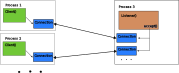
\includegraphics[width=\textwidth]{listener_client.pdf}
    \caption{Relationships between Listeners, Clients and Connections}
\end{figure}

The example below shows a simple echo server -- a server that simply sends back to the client what it receives. It will only accept connections from the local computer on the port 6000. First, the listener object is created using the \ls{with} statement, which is then used to start a separate thread which accepts the connections and responds to clients. The main thread will simply wait for the signal to quit. If we are supposed to quite, close the listener (we also need to unblock the \ls{accept()} which would wait forever) and quit. Note that the passwords are optional, if you do not specify the \ls{authkey} for the \ls{Listener}, you also do not have to specify it for \ls{Client}.

The client is in comparison much simpler. Simply connect to the listener with known address, port and password, and you can start sending and receiving data. Note that \ls{send()} and \ls{recv()} pickle and unpickle (recall pickling from \ls{.npy} files), so almost all Python-objects can be sent.

To test the example below, run \verb|python server.py| in one console and \verb|python client.py| in another.

\ls{server.py}:
\lstinputlisting{../example_code/ipc_server.py}

\ls{client.py}
\lstinputlisting{../example_code/ipc_client.py}

To allow connections from the network, simply specify the Listener address as \ls{''} (empty string) and the connect with the client to the IP address of the computer running the listener process. Note that pickling and unpickling in \ls{send()} and \ls{recv()} can lead to potential security issues, so it is best to use a password if accepting connections over the network.

\begin{exercise}
A server is running on computer with IP address \verb|<IP>|, on port \verb|<PORT>| with password \verb|<PASSWORD>|. This server is controlling a Pico by directly sending whatever string it receives to the pico and sending the response from the pico back. Connect to this server with a client, send the command \verb|*IDN?| to query the instrument's identification and blink an LED if the response is correct.
\end{exercise}

\verb|instrument_server.py|:
The code accepts the connections in a separate thread. For each connection it accepts, it starts a new client handler thread. All client handler threahds share the same pico, so we have to lock it appropriately before attempting communication, because another client can interrupt us at any moment. The server quits when it receives KeyboardInterrupt (Ctrl-C) 
\lstinputlisting{../example_code/instrument_server.py} %

\subsubsection{Real use case in a lab}
In Fig.~\ref{fig:networking-usecase} is a photo of a single computer which controls three experiments connected to two different experimental setups. Each experiment belongs to a different student, who might need to run and modify their measurement Python scripts at the same time, so simple remote desktop sharing is not available.

We ended up using an instrument server similar to the simplified example above, which allowed the students to run the measurement scripts on any computer on the same network, even on their own laptops.

\begin{figure}
    \label{fig:networking-usecase}
    TODO
    \caption{Single computer controlling multiple experiments.}
\end{figure}
% \newpage
\section{Řešení diferenciálních rovnic}
\subsection{Počáteční úlohy}
Počáteční úlohy jsou diferenciální rovnice tvaru
\begin{equation}
    \label{eq:ivp}
    \diff{\bv y}{t} = \bv f(\bv y, t),
\end{equation}
kde $\bv y$ je vektor, $t$ je čas a $\bf f$ je libovolná funkce spolu s počáteční podmínkou $\bv y(t=0) = \bv y_0$. Všimněte si, že rovnice je vždy zapsána ve tvaru obyčejné diferenciální rovnice prvního řádu. Diferenciální rovnici libovolného řádu však lze přepsat na rovnici prvního řádu nastavením vektoru $\bv y = (y(t), y'(t), y''(t), \dots)$. Například Newtonův pohybový zákon, $\ddot x = F/m$ by odpovídal $\bv y = (x, \dot x)$ a $\bv f = (\dot x, F/m)$.

Tyto typy rovnic se obvykle řeší \emph{časovým krokováním}: víme-li, že $\bv y(t=0) = \bv y_0$, vypočítáme $\bv y(\dd t) \approx \bv y(0) + \bv f(\bv y(0), 0)\dd t$; $\bv y(2\dd t) \approx \bv y(\dd t) + \bv f(\bv y(\dd t), \dd t)\dd t$ $\dots$. Toto časové krokování se nazývá \emph{Eulerova} metoda a obecně vyžaduje malý časový krok, aby byla přesná a numericky stabilní.\footnote{Numerická \emph{nestabilita} je tendence chyby (tj. rozdílu mezi skutečným řešením a jeho numerickou aproximací) divoce oscilovat nebo růst do nekonečna.} Existuje mnoho schémat časového krokování, která jsou přesnější a stabilnější než základní Eulerova metoda. Přesnost metody se často kvantifikuje pomocí notace velké O, tj. Eulerova metoda je $O(\dd t)$, neboli metoda prvního řádu, což znamená, že pokud zmenšíme časový krok $\dd t$ na polovinu, zmenšíme na polovinu i chybu v každém kroku. Velmi běžné jsou explicitní metody Runge-Kutta, z nichž 4. řád (s přesností $O(\dd t^4)$) je pravděpodobně nejběžnější, tj. pokud zmenšíme časový krok na polovinu, chyba se sníží 16krát.

Runge-Kuttova metoda čtvrtého řádu (RK4) počítá $y(t + \dd t)$ z $y(t)$ jako
\begin{equation}
    \label{eq:RK4} %
    y(t + \dd t) = y(t) + \frac{\dd t}{6}\left(k_1 + 2k_2 + 2k_3 + k_4\right),
\end{equation}
where
\begin{equation}
    \begin{aligned}
        k_1 &= f(y_t, t)\\
        k_2 &= f\left(y_t + \frac{1}{2}\dd t k_1, t + \frac{1}{2}\dd t\right)\\
        k_3 &= f\left(y_t + \frac{1}{2}\dd t k_2, t + \frac{1}{2}\dd t\right)\\
        k_4 &= f(y_t + k_3 \dd t, t + \dd t).
    \end{aligned}
\end{equation}
Všimněte si, že pro každý časový krok musí být funkce $f$ vyhodnocena 4krát a výpočet je asi 4krát pomalejší než Eulerova metoda. Existují také metody časového krokování, které místo toho, aby trvaly 4krát déle, zabírají 4krát více místa (např. rodina metod Adams-Bashforth), které k odhadu dalšího kroku používají poslední čtyři kroky v historii $y(t)$.

Metoda RK4 pro problém typu \eqref{eq:ivp} je implementována v \verb|SciPy| v \ls{scipy.integrate.solve_ivp()}. \ls{solve_ivp()} očekává funkci $f(t, y)$, která přebírá čas a stavový vektor a vrací časovou derivaci stavového vektoru, počáteční podmínku a časový rozsah, ve kterém se má vývoj počítat.

Výpočet může také sledovat \emph{události} -- typicky signál, že by měl výpočet skončit. Jedná se o funkce času a stavového vektoru, které při výskytu události \emph{změní znaménko}. Událost lze učinit terminální (tj. když k události dojde, výpočet by se měl zastavit) jednoduchým nastavením atributu \ls{terminal} funkce na \ls{True}. Pamatujte, že funkce jsou objekty a jejich atributy můžeme nastavovat, jak se nám zlíbí (podobně jako \ls{self.attribute = value} při práci s třídami).

\textbf{Příklad}: Vypočítejte balistickou trajektorii míče kopnutého pod úhlem 45$^\circ$ s počáteční rychlostí 3 m/s ve směru $x$ i $y$. Balistická trajektorie je trajektorie projektilu vrženého v prostředí (např. ve vzduchu), které na pohyb působí nelineární odporovou silou tvaru
\begin{equation}
    \bv F_d = -\frac{1}{2}A|\bv v|\bv v \rho \mathrm{CD},
\end{equation}
kde $\bv v$ je rychlost projektilu, $A$ je plocha průmětu projektilu ve směru pohybu, $\rho$ je hustota prostředí a CD je koeficient odporu, $\mathrm{CD}\approx0.47$ pro míč.

\textbf{Řešení:}
Úplný kód je k dispozici v \ls{ivp_ballistic.py}. Nejprve naimportujeme potřebné moduly a definujeme potřebné konstanty
\lstinputlisting[linerange={1,2,3,4,5,6,7,8,9,10}]{../example_code/ivp_ballistic.py}

Dále definujeme funkci $f$. Vezmeme stavový vektor $\bv x = (x, y, v_x, v_y)$, který reprezentuje vektory polohy i rychlosti. Funkce musí vracet časovou derivaci tohoto 4-složkového stavového vektoru
\lstinputlisting[linerange={12-25}]{../example_code/ivp_ballistic.py}

Dále definujeme událost, která bude indikovat, že míč dopadl na zem, a učiníme ji terminální, protože nechceme, aby výpočet pokračoval za tento bod
\lstinputlisting[linerange={30-34}]{../example_code/ivp_ballistic.py}

Nyní máme vše, co potřebujeme k výpočtu balistické trajektorie. Nastavíme časový rozsah výpočtu na $(0, 10)$, kde 10 je jen libovolně velký čas, výpočet bude zastaven událostí dopadu. Předáme také další argumenty, koeficient odporu, prostřednictvím obvyklého klíčového argumentu \ls{args=}. Nakonec také požádáme o \ls{dense_output}, který vrátí interpolační objekt (\ls{solution.sol} níže) pro reprezentaci řešení. To je užitečné, protože \ls{solve_ivp} používá adaptivní velikost časového kroku $\dd t$ (tj. když jsou derivace malé a pomalu se mění, časový krok je větší), takže pokud chceme rovnoměrně vzorkované řešení, musíme ho interpolovat. S vráceným řešením použijeme čas události k vytvoření rovnoměrně vzorkovaného časového pole a vrátíme interpolovanou trajektorii.

Nakonec vypočítáme trajektorii s odporem vzduchu a bez něj a vykreslíme ji. Použijeme mírně nenulovou počáteční podmínku v poloze $y$, abychom se vyhnuli spuštění události na začátku.
\lstinputlisting[linerange={36-}]{../example_code/ivp_ballistic.py}

% \lstinputlisting{../example_code/ivp_ballistic.py}
\begin{center}
    \includegraphics[width=0.6\linewidth]{ballistic.png}
\end{center}

\begin{exercise}
    Vypočítejte pohyb harmonického oscilátoru s hmotností $m=1$ kg a tuhostí pružiny $k=1$ N/m s počáteční polohou $x_0 = 1$ m a počáteční rychlostí $v_0 = 0$ m/s. Vykreslete polohu a rychlost jako funkci času pro $t \in [0, 10]$ s časovým krokem $\dd t = 0.1$ s.
\end{exercise}

\begin{exercise}
    Simulujte populační dynamiku predátorů a kořisti (lišky $F$ a králíci $R$) pomocí Lotka-Volterra modelu:
    \begin{equation*}
        \begin{aligned}
            \frac{\dd R}{\dd t} &= aR - bFR\\
            \frac{\dd F}{\dd t} &= dFR - cF
        \end{aligned}
    \end{equation*}
    s $a = 2/3$, $b = 4/3$ a $c = d = 1$. Vykreslete $R(t)$ a $F(t)$ a trajektorii ve fázovém prostoru $R-F$.
\end{exercise}

\begin{exercise}
    Simulujte Lorenzův systém (první řádně prostudovaný příklad deterministického chaosu) daný rovnicemi
    \begin{equation*}
        \begin{aligned}
            \frac{\dd x}{\dd t} &= \sigma (y - x)\\
            \frac{\dd y}{\dd t} &= x(\rho - z) - y\\
            \frac{\dd z}{\dd y} &= xy - \beta z,
        \end{aligned}
    \end{equation*}
    s $\sigma = 10$, $\rho = 28$ a $\beta = 8/3$. Vykreslete trajektorii $x$, $y$, $z$ ve 3D prostoru.
\end{exercise}

\begin{syntax}[3D grafy]
Matplotlib podporuje 3D vykreslování. V posledních verzích matplotlibu je jednoduchý 3D graf čáry dané poli \ls{x}, \ls{y} a \ls{z} velmi jednoduchý:
\begin{lstlisting}
fig3d = plt.figure()
ax3d = fig3d.add_subplot(projection='3d')
ax3d.plot(x, y, z, lw=0.5)
\end{lstlisting}
\end{syntax}

\subsection{Okrajové úlohy}
Okrajové úlohy jsou diferenciální rovnice tvaru
\begin{equation}
    \label{eq:bvp}
    F(\bv y, x) = 0
\end{equation}
kde $F$ je nějaká funkce, která definuje náš problém a závisí na neznámé funkci samotné a jejích derivacích, $\bv y$ je neznámá funkce $x \in [a,b]$ podléhající okrajovým podmínkám $B(y_a, y_b) = 0$. Zde je neznámá funkce funkcí prostoru, nikoli času, a potřebujeme znát řešení "všude" najednou. Numerické algoritmy obvykle začínají nějakým počátečním odhadem a poté iterativně optimalizují řešení $\bv y$ tak, aby splňovalo rovnici \eqref{eq:bvp} při zachování okrajových podmínek.

Řešení 1D (dimenze $x$) okrajových úloh je implementováno v \verb|SciPy| v \ls{scipy.integrate.solve_bvp}, což také umožňuje nalézt neznámé parametry, pro které může řešení existovat (viz příklad níže). Pro vícerozměrné problémy obvykle musíte použít specializovaný balíček nebo si napsat vlastní.

Vyřešíme jednoduchý příklad 1D Schrödingerovy rovnice:\\
\textbf{Příklad} Vypočítejte vlnové funkce a energetické hladiny částice v nekonečné potenciálové jámě s dodatečným potenciálem $V(x)$ uvnitř jámy.

Stavy kvantové částice jsou popsány stacionární Schrödingerovou rovnicí
\begin{equation}
    \label{eq:sch}
    E\psi = -\frac{\hbar^2}{2m}\frac{\dd^2\psi}{\dd x^2} + V(x)\psi,
\end{equation}
kde $m$ je hmotnost částice, $\psi$ je vlnová funkce částice a $E$ je energie. Počítejte v "atomových jednotkách", $\hbar = 1$, $m=1$ a potenciál tvaru znázorněného na obr.~\ref{fig:potential}, tj. $V(|x| > 1) = \infty$ a $V(|x| < 0.1) = 10)$ a jinde $V=0$.
\begin{figure}[h!]
    \centering
    \label{fig:potential}
    \includegraphics[width=0.5\linewidth]{sch_potential.pdf}
    \caption{Potenciál pro Schrödingerovu rovnici \eqref{eq:sch}.}
\end{figure}

\textbf{Řešení:} Úplný kód je k dispozici v \ls{bvp_schrodinger.py}.

Začněte importováním všeho, co potřebujeme, definujte konstanty \ls{w}, šířku bariéry a \ls{dh} výšku bariéry a samotnou funkci potenciálu. O nekonečné stěny v $x=\pm 1$ se postarají okrajové podmínky.
\lstinputlisting[linerange={6,7,8,9,10,11,12,13,14,15,16,17,18,19,20,21}]{../example_code/bvp_schrodinger.py}

Dále definujte funkci $F$ z \eqref{eq:bvp}. Přepíšeme Schrödingerovu rovnici \eqref{eq:sch} na
\begin{equation}
    \frac{\dd^2\psi}{\dd x^2} = 2m(V(x) - E)\psi,
\end{equation}
a neznámá funkce $\bv y$ je pak $(\psi, \dd \psi/\dd x)$. Nakonec musíme také najít neznámý parametr $E$. Funkce $F$ může záviset na vektoru neznámých parametrů, které \ls{solve_bvp()} najde spolu s neznámou funkcí. V tomto případě je to jen energie.
\lstinputlisting[linerange={23-29}]{../example_code/bvp_schrodinger.py}

Dále je funkce reprezentující okrajové podmínky. Jedná se o libovolnou funkci hodnoty neznámé funkce na hranicích a neznámých parametrů, kterou \ls{solve_bvp} udržuje na nule. Musíme vrátit vektor velikosti 2 (tj. počet hranic) + počet neznámých parametrů. V našem případě jednoduše chceme, aby vlnová funkce byla na nekonečné stěně nulová. Třetí okrajová podmínka je libovolná a jejím účelem je jednoduše zajistit, aby nalezené řešení nebylo identicky 0.
\lstinputlisting[linerange={35-36}]{../example_code/bvp_schrodinger.py}
Číslo ve třetí podmínce je libovolné, protože řešení poskytnuté \ls{solve_bvp} není normalizováno.

Dále musíme vytvořit počáteční podmínku, jak pro vlnovou funkci, tak pro energii, aby ji řešitel mohl optimalizovat. Všimněte si, že původní Schrödingerova rovnice \eqref{eq:sch} má nekonečně mnoho řešení. K jakému řešení \ls{solve_bvp()} skutečně konverguje, je dáno touto počáteční podmínkou. Nejprve vytvoříme mřížku, tj. body v prostoru $x$, které jsou argumentem vlnové funkce, a vytvoříme jednoduchý odhad vlnové funkce, která je všude nulová a nenulová v jednom bodě mimo střed, abychom konvergovali k řešení lokalizovanému v jedné polovině potenciálové jámy. Pamatujte, že úplná počáteční podmínka je vlnová funkce a její gradient, takže \ls{y_0} je 2D pole velikosti 2 $\times$ délka \ls{x}.
\lstinputlisting[linerange={38-50}]{../example_code/bvp_schrodinger.py}

Pro energii jednoduše použijeme energii základního stavu částice v jednoduché nekonečné potenciálové jámě.
\lstinputlisting[linerange={53}]{../example_code/bvp_schrodinger.py}

Nakonec máme vše, co potřebujeme k zavolání \ls{solve_bvp()}. Fyzikálně nejzajímavější částí je pravděpodobnost nalezení částice v poloze $x$, která je dána $|\psi(x)|^2$, takže tu vykreslíme. Abychom byli přesní, měli bychom také normalizovat vlnovou funkci tak, aby $\int |\psi(x)|^2 \dd x = 1$, nicméně, protože nepočítáme žádné kvantově mechanické střední hodnoty a zajímá nás pouze tvar rozdělení, vykreslíme ji tak, jak je, spolu s potenciálem a nalezenou energií.
\lstinputlisting[linerange={56, 65-74}]{../example_code/bvp_schrodinger.py}

\subsection{GPU akcelerace}
Některé typy fyzikálních problémů lze efektivně počítat na grafických kartách (GPU). Jedná se o problémy, které zahrnují mnoho nezávislých výpočtů, které lze spouštět paralelně. Prototypickým příkladem je gravitační problém $N$ těles: vypočítejte pohyb $N$ planet se stejnou hmotností $m$, které na sebe vzájemně působí pouze gravitací.

Pro zjednodušení vykreslování budeme uvažovat 2D případ. Celková síla působící na planetu $j = 1\dots N$ je
\begin{equation}
    \bv F_j = Gm^2\sum_{k\neq j}\frac{\bv r_k - \bv r_j}{|\bv r_k - \bv r_j|^3}, %
\end{equation}
kde $G$ je gravitační konstanta a $\bv r_k$ jsou polohy planet. Pohyb planety je pak dán jednoduše $m\ddot{\bv r_j} = \bv F_j$ a mohli bychom použít \ls{solve_ivp()} jako předtím. Tento problém se však stává vědecky zajímavějším pro velký počet planet, kde by se \ls{solve_ivp()} rychle zastavilo. Proto chceme využít rychlé GPU.

Výpočet bude opět probíhat v krocích: budeme mít uloženy všechny polohy a rychlosti planet. V každém kroku vypočítáme celkovou sílu působící na všechny planety a poté pro zjednodušení aktualizujeme polohy a rychlosti pomocí Eulerova krokování. Výpočet zahrnuje $N^2$ výpočtů sil mezi planetami, které jsou na sobě nezávislé. Naším cílem je použít GPU k jejich paralelnímu spuštění.

The full code is \verb|example_code/taichi/gravity.py|

\subsubsection{Nastavení prostředí}
K akceleraci výpočtů z Pythonu budeme používat knihovnu \ls{taichi}, která má tu výhodu, že je poměrně jednoduchá, vypadá velmi podobně jako standardní kód v Pythonu a umožňuje používat buď GPU, nebo CPU se stejným kódem, takže si níže uvedený kód můžete vyzkoušet, i když v počítači nemáte dedikovanou GPU. Taichi bohužel vyžaduje Python verze 3.10, což s největší pravděpodobností není verze, kterou máte nainstalovanou. Nechceme systém zahlcovat více verzemi Pythonu, proto použijeme \emph{virtuální prostředí}, abychom měli izolovanou instalaci Pythonu s vlastní verzí a balíčky.

Nejjednodušší způsob, jak spravovat virtuální prostředí, je pomocí nástroje \ls{uv} \url{https://docs.astral.sh/uv/getting-started/installation/}. V systému Windows spusťte instalační příkazy v prostředí Windows Powershell.

Jakmile je \ls{uv} nainstalováno, vytvořte prázdný adresář, nazvěme ho "gravity", přejděte do něj v příkazovém řádku a spusťte
\begin{lstlisting}[language=bash]
uv venv -p 3.10
\end{lstlisting}
což vytvoří virtuální prostředí s Pythonem verze 3.10. Měli byste vidět výstup, který vypadá podobně jako
\begin{verbatim}
Using CPython 3.10.16 interpreter at: /usr/bin/python3.10
Creating virtual environment at: .venv
Activate with: source .venv/bin/activate
\end{verbatim}
Aktivujte virtuální prostředí příkazem z posledního řádku. Váš příkazový řádek by nyní měl zobrazovat virtuální prostředí, např. na mém linuxovém počítači
\begin{verbatim}
(gravity) emil@nt202 ~/gravity $
\end{verbatim}
Toto je čistý stůl, kam musíme nainstalovat všechny potřebné knihovny Pythonu. Budeme potřebovat pouze \ls{taichi} a \ls{matplotlib} (a jejich závislosti), které můžeme nainstalovat jednoduše pomocí
\begin{lstlisting}
uv pip install taichi matplotlib
\end{lstlisting}
a nyní máme vše, co potřebujeme k psaní a spouštění kódu taichi. Musíme však mít aktivované prostředí, jinak používáme systémový python, který o knihovně taichi neví.

\subsubsection{Testování instalace}
Spustěte Python v příkazovém řádku zadáním \ls{python} a zadejte následující kód pro otestování instalace taichi:
\begin{lstlisting}
>>> import taichi as ti
[Taichi] version 1.7.4, llvm 15.0.4, commit b4b956fd, linux, python 3.10.19
>>> ti.init(ti.gpu)  # alebo ti.cpu
[W 12/02/25 13:29:07.195 37705] [cuda_driver.cpp:load_lib@36] libcuda.so lib not found.
[Taichi] Starting on arch=vulkan
\end{lstlisting}
Pokud vidíte podobný výstup, je vše v pořádku. Varování o chybějící knihovně \ls{libcuda.so} je v pořádku, pokud nemáte NVIDIA GPU. Taichi se pokusí použít Vulkan na GPU AMD nebo Intel, nebo pokud není k dispozici žádná GPU, použije CPU.

\subsubsection{GPU Kernely}
Taichi nám umožňuje přesunout specifické funkce ke spuštění na GPU. S těmito funkcemi se zachází odlišně od zbytku kódu v Pythonu a nazývají se \emph{kernely}. Napíšeme dva kernely, jeden pro výpočet sil a druhý pro Eulerovo krokování. Data budeme ukládat do polí numpy -- není to nejrychlejší způsob (taichi umí paměť využívat efektivněji, viz dokumentace taichi pro optimalizovanější verzi), ale je to nejjednodušší.

Importujeme taichi a požádáme ho o použití GPU, pokud je to možné, pomocí
\begin{lstlisting}
import taichi as ti
ti.init(ti.gpu)
\end{lstlisting}
Tím se použije v pořadí podle priority NVIDIA CUDA, Vulkan na GPU od AMD nebo CPU.

The Euler stepping kernel looks like this
\lstinputlisting[linerange={49-59}]{../example_code/taichi/gravity.py}
Označíme, že funkce je kernel, pomocí dekorátoru \ls{ti.kernel}. Funkce přebírá čtyři argumenty -- polohy planet \ls{rs}, rychlosti \ls{vel} a zrychlení \ls{acc}, což jsou pole numpy 64bitových floatů tvaru \ls{(N,2)} ($N$ planet a dvě souřadnice) a časový krok \ls{dt}, což je jednoduchý float.

Uvnitř funkce vypadá poměrně obyčejně, nicméně běží uvnitř GPU a vnější cyklus for ve skutečnosti není cyklus, ale iterace se provádějí co nejvíce paralelně. Existují určitá omezení -- například nesmíte \ls{break} z vnějšího cyklu. Vnitřní cyklus (\ls{for k in range(2)}) běží jako běžný sekvenční cyklus for. Nic nevracíme, ale spíše upravujeme vstupní pole.

Zajímavějším kernelem je výpočet zrychlení (nebo sil), který vypadá takto
\lstinputlisting[linerange={14-46}]{../example_code/taichi/gravity.py}

Náš problém je relativně jednoduchý, tzv. \emph{trapně paralelní}\footnote{Toto je skutečný termín používaný v informatice.}, protože výpočty jsou na sobě zcela nezávislé. GPU jsou schopny rychle spouštět mnoho úloh paralelně, protože neumožňují synchronizaci (nebo jen ve velmi omezené formě). To znamená, že i přes paralelní spouštění mnoha věcí nemáme žádný mechanismus podobný \ls{Lock()} z multithreadingu. Pokud tedy iterace cyklu na sobě závisí, stává se vyhýbání se souběhovým stavům poněkud složitější. Představte si například, že některé planety jsou z hmoty a některé z antihmoty a pokud se k sobě příliš přiblíží, anihilují. Mohli bychom to implementovat například jako
\begin{lstlisting}
for j in range(N):
    for k in range(N):
        if planet_is_alive(j) and planet_is_alive(k):
            if distance(j,k) < annihilation_distance:
                annihilate(j,k)
\end{lstlisting}
To by bylo v pořádku, kdyby cykly byly sekvenční. Když však vnější cyklus běží paralelně, mohli bychom se dostat do situace, kdy máme planety $j=1$ (hmota) a $k=2, 3$ (antihmota), které jsou všechny blízko sebe. Protože kontrola na řádku 3 může používat stará data, mohli bychom skončit spuštěním jak \ls{annihilate(1,2)}, tak \ls{annihilate(1,3)} a tím zvýšit poměr hmoty k antihmotě ve vesmíru.

\subsubsection{Použití kernelů}
K reprezentaci stavu simulace -- poloh a rychlostí planet a času -- použijeme jednoduchou třídu. Jako počáteční podmínku použijeme náhodné polohy ve 2D s normálním rozdělením kolem počátku a rotaci tuhého tělesa pro rychlosti s nějakou počáteční úhlovou rychlostí. Třída bude mít pouze dvě metody, které volají dva kernely, které jsme napsali výše,
\lstinputlisting[linerange={61-88}]{../example_code/taichi/gravity.py}

Nakonec vytvoříme simulaci s 5000 planetami, vykreslíme animaci v reálném čase pomocí matplotlib a periodicky ukládáme obrázek
\lstinputlisting[linerange={91-130}]{../example_code/taichi/gravity.py}

Asi po minutě běhu na CPU Intel Core i7-7700 (poměrně staré CPU) se počáteční gaussovské rozdělení planet vyvine do zajímavé struktury
\begin{center}
    \includegraphics[width=0.5\linewidth]{gravity.png}
\end{center}

\begin{exercise}
    Implementujte výpočet Mandelbrotovy množiny pomocí taichi.
\end{exercise}
% \newpage
\section{What didn't fit}

\subsection{PID algorithm}
TODO

\subsection{Symbolic mathematics}
TODO: sympy

% \section{Image processing}
% TODO, \ls{opencv}

% \section{Some AI crap?}
% TODO \ls{scikit-learn}

\newpage
\appendix
% %Appendices
\section{Linear Harmonic Oscillator}
\label{sec:lho}
A linear harmonic oscillator with friction is described by a dynamical equation
\begin{equation}
    \label{eq:lho}
    \ddot x + \omega_0^2 x + \gamma\dot x = F(t)/m,
\end{equation}
where $m$ is the oscillator mass, $\omega_0$ is the resonance frequency, $\gamma$ the friction coefficient and $F(t)$ the external force. Assuming that the force has the form $F(t) = \Re(\tilde F e^{i\omega t})$ and that the solution has the form $x(t) = \Re(\tilde x e^{i\omega t})$ (or applying the Fourier transform to both sides of the equation) we get by simple rearranging
\begin{equation}
    \tilde x = \frac{1}{m}\frac{\tilde F}{\omega_0^2 - \omega^2 + i\gamma\omega} = \chi(\omega)\tilde F,
\end{equation}
where $\chi(\omega)$ is called susceptibility.

Since Eq.~\ref{eq:lho} is a linear equation, the response to a sum of forces will be the sum of responses to each force.

\section{Setting up communication with instruments}
\label{sec:pico}
We will use VISA library to talk to instruments. To talk to the Raspberry Pi Pico we will use a Python implementation of the library, for which we need to install at least \ls{pyvisa, pyvisa-py} and \ls{pyusb} using
\begin{lstlisting}[language=bash]
    pip install pyvisa pyvisa-py pyusb
\end{lstlisting}
which you should run in a command line which is aware of the python installation (e.g., Anaconda Propmt if on Windows with Anaconda Python distribution). On Linux you should also add yourself to the \ls{dialout} group (do not forget the \ls{-a} switch),
\begin{lstlisting}[language=bash]
    sudo usermod -a <your username> -G dialout 
\end{lstlisting}
and log out and log in.

To test the installation run the \ls{pyvisa-info} from the command line. A bunch of information should be printed out, look for line that looks like
\begin{lstlisting}
    USB INSTR: Available via PyUSB (1.2.1). Backend: libusb1
\end{lstlisting}

Next, create a Python script \ls{list_resources.py} with the following code
\lstinputlisting{../example_code/list_resources.py}
and run it. It should list either nothing or a few COM (or tty on Linux) ports. Next connect the Pico and run the program again, a new address should appear, that is the address we will use to communicate with the Pico.

Next, run the following code, replacing \ls{"ASRL/dev/ttyACM0::INSTR"} with the address you found in the previous step.
\lstinputlisting{../example_code/idn.py}
The program should print "PICO" and quit without error.

For more full-featured implementation of visa you may consider the implementation from \href{https://www.ni.com/en/support/downloads/drivers/download.ni-visa.html#548367}{National Instruments} (NI). The NI-VISA library is free, but not open source and registration is required. Linux support is also limited to out-of-date kernels.

\subsection{Supported commands}
\begin{tabular}{p{15cm}}
    \textbf{*IDN?}\\
    Query identification string. Should reply PICO.
    \\\hline
    \textbf{:LED n m}\\
    Turns the LED $n$ on (m=1) or off (m=0). The LED number $n = 0 \dots 4$, red LED is 0.
    \\\hline
    \textbf{:READ:P?}\\
    Reads the pressure in Pa.
    \\\hline
    \textbf{:READ:T?}\\
    Returns the temperatures as $100T$ where $T$ is the temperature in $^\circ$C.
    \\\hline
    \textbf{:READ:PT?}\\
    Reads both temperature and pressure
    \\\hline
    \textbf{:READ:ACC?}\\
    Reads the accelerometer. Returns three space-separated values in the range -32768 to 32768 which maps to $-2g$ to $2g$.
    \\\hline
    \textbf{:READ:GYR?}\\
    Reads the gyroscope. Returns three space-space separated values in the range -32768 to 32768 which maps to $-500^\circ$/s to $500^\circ$/s.
\end{tabular}

\subsection{Hacking the firmware}
The source code of the program running on the Pico is available \href{https://bitbucket.org/emil_varga/picolab/src/master/}{here}. To compile it, you need to set up Pico SDK, follow the instructions \href{https://www.raspberrypi.com/documentation/microcontrollers/c_sdk.html}{here}.

Alternatively you can use MicroPython to run Python code on the Pico directly, follow the instructions \href{https://www.raspberrypi.com/documentation/microcontrollers/micropython.html#what-is-micropython}{here} for set up. 

LEDs are wired to GP0 -- GP4 pins and the sensors are connected to the I2C0 controller on pins 16 and 17.

\section{Basics of git version control system}
\label{sec:git}
TODO
\end{document}


\end{document}